\section{Эпитаксиальный синтез наногетероструктур}

\begin{frame}[plain, noframenumbering]
	\begin{center}
		\Huge
		Эпитаксиальный синтез наногетероструктур
	\end{center}
\end{frame}

\begin{frame}
	\frametitle{Эпитаксиальные A\textsuperscript{III}B\textsuperscript{V} гетероструктуры на Si}
	\begin{itemize}
		\item Уменьшение себестоимости производства оптоэлектронных приборов
		\item Замена электронных компонентов интегральных схем на оптические
	\end{itemize}
\end{frame}

\begin{frame}
	\frametitle{Эпитаксиальные наногетероструктуры A\textsuperscript{III}B\textsuperscript{V}}
	\begin{itemize}
		\item Релаксация напряжений и низкая концентрацию структурных дефектов
		\item Дополнительные возможности для зонного проектирования
		\item Синтез нестабильных кристаллографических фаз
		\item Электронное и оптическое ограничение
		\item Зависимость взаимодействия со светом от морфологии
	\end{itemize}
\end{frame}

\section{Влияние подготовки поверхности на формирование GaN наноструктур}

\begin{frame}[plain, noframenumbering]
	\begin{center}
		\Huge
		Влияние подготовки поверхности на формирование эпитаксиальных GaN наноструктур
	\end{center}
\end{frame}

\begin{frame}
	\frametitle{Нитридация Ga капель}
	\centering
	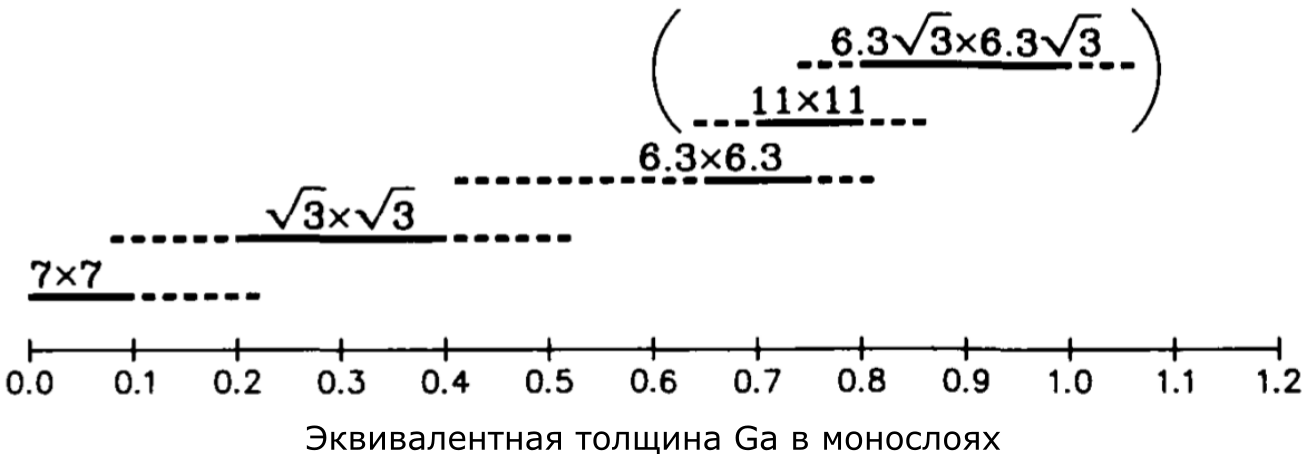
\includegraphics[width=0.8\linewidth]{Image_12} \\
	\vfill
	\begin{minipage}[t]{0.4\linewidth}
		\center{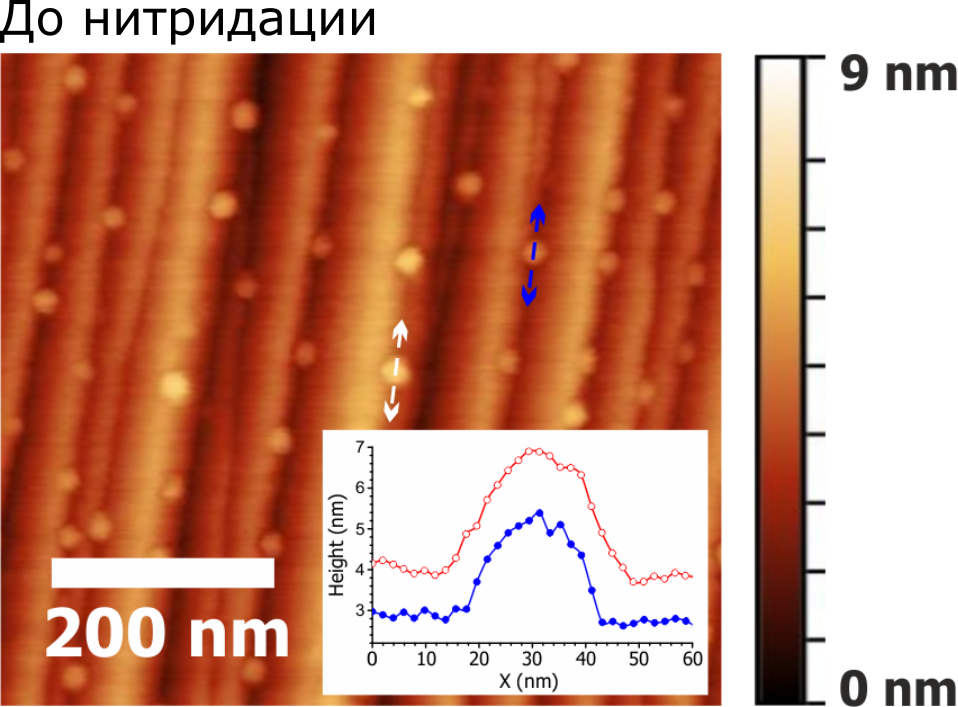
\includegraphics[width=1\linewidth]{Image_13_1}}
	\end{minipage}
	\begin{minipage}[t]{0.4\linewidth}
		\center{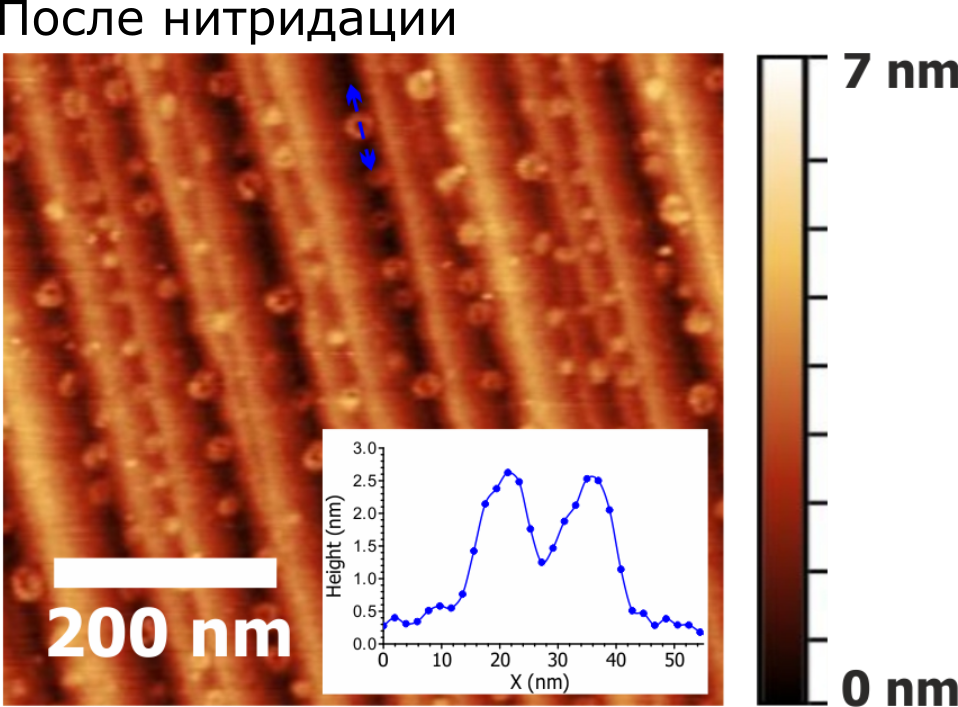
\includegraphics[width=1\linewidth]{Image_13_2}}
	\end{minipage}
\end{frame}

\begin{frame}
	\frametitle{GaN триподы}
	\centering
	\begin{minipage}[t]{0.2\linewidth}
		\center{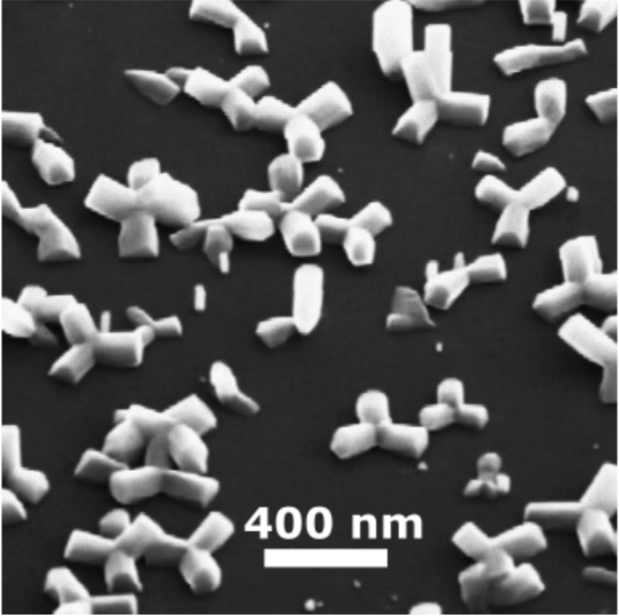
\includegraphics[height=0.20\textheight]{Image_14_1}}
	\end{minipage}
	\begin{minipage}[t]{0.2\linewidth}
		\center{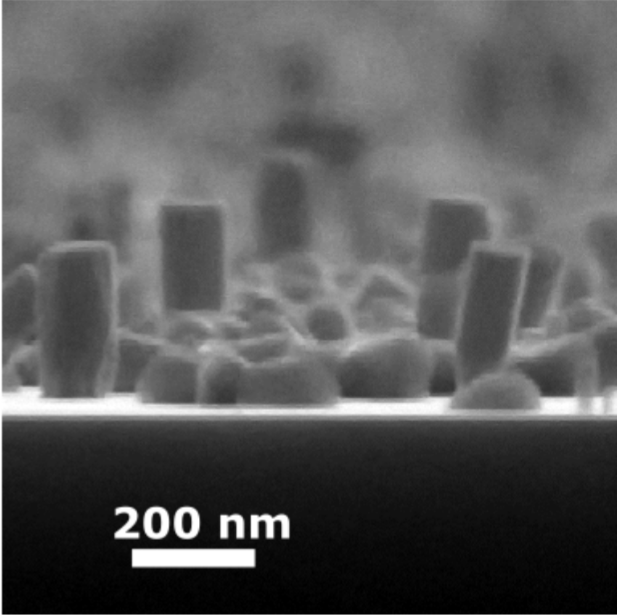
\includegraphics[height=0.20\textheight]{Image_14_2}}
	\end{minipage}
	\begin{minipage}[t]{0.2\linewidth}
		\center{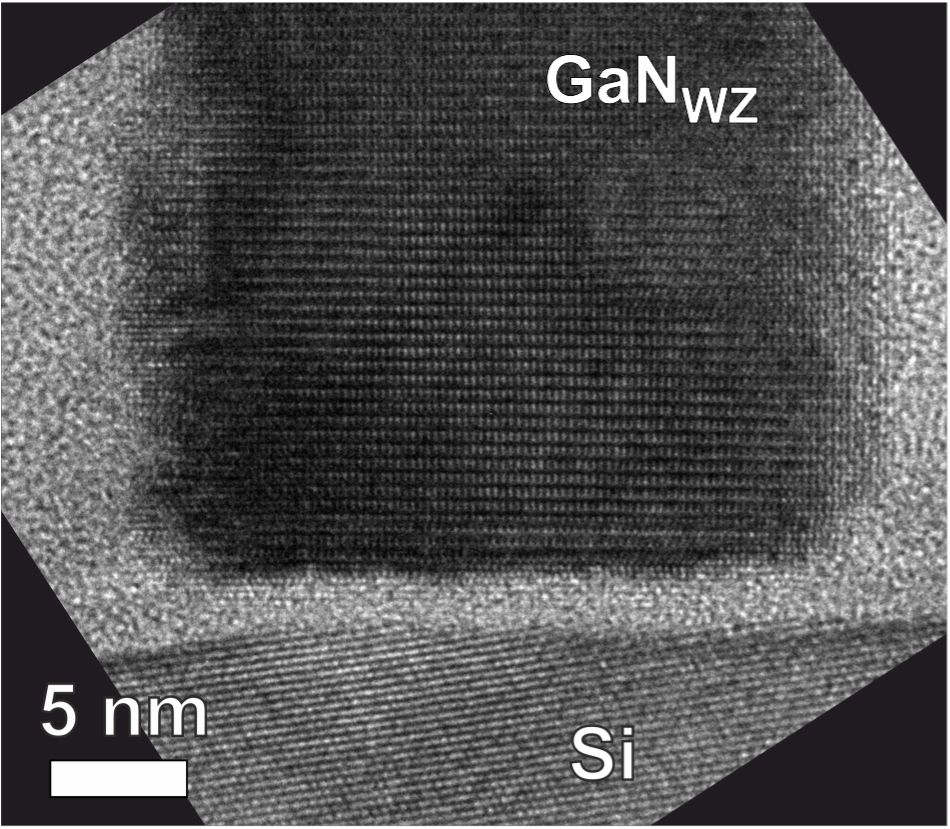
\includegraphics[height=0.20\textheight]{Image_15_1}}
	\end{minipage}
	\begin{minipage}[t]{0.2\linewidth}
		\center{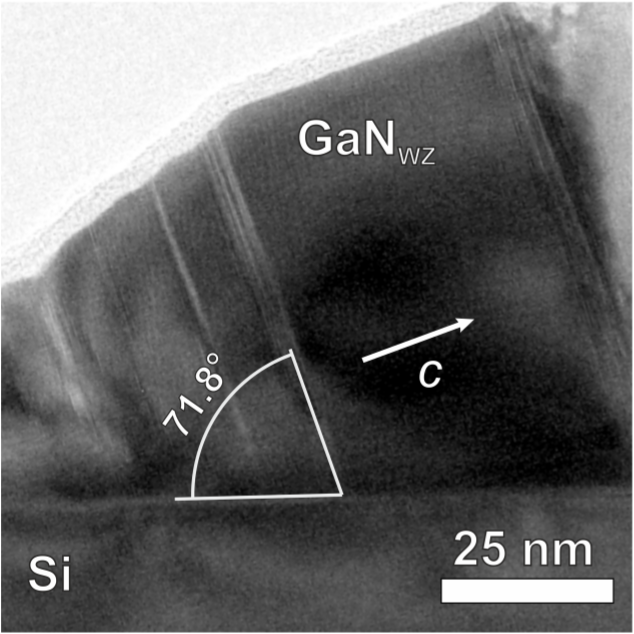
\includegraphics[height=0.20\textheight]{Image_15_2}}
	\end{minipage}
	\bigskip
	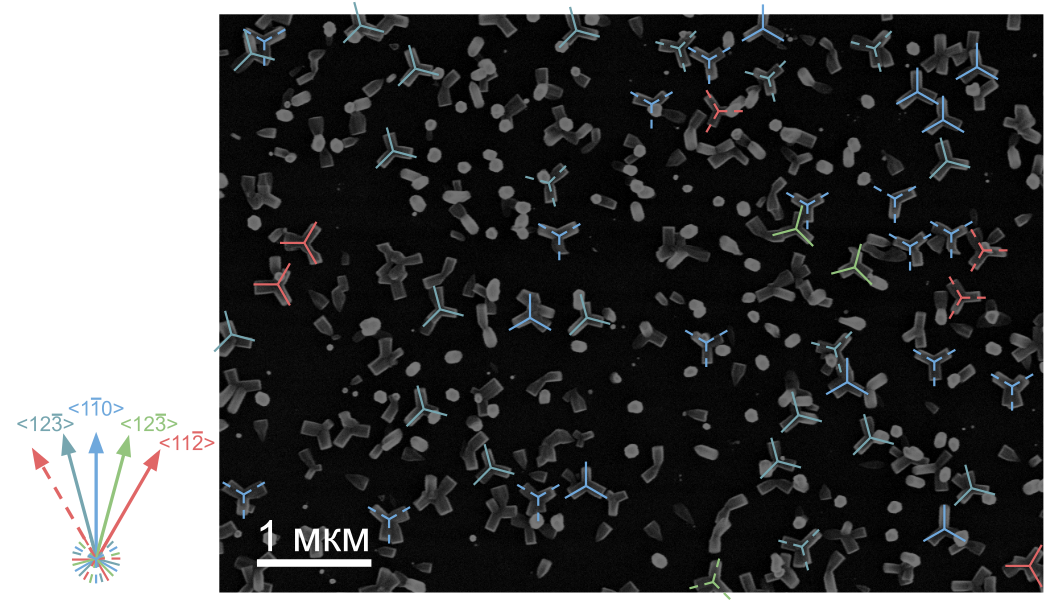
\includegraphics[width=0.8\linewidth]{Image_14_3}
\end{frame}

\begin{frame}
	\frametitle{Кристаллическая структура триподов}
	\centering
	\begin{minipage}[t]{0.25\linewidth}
		\center{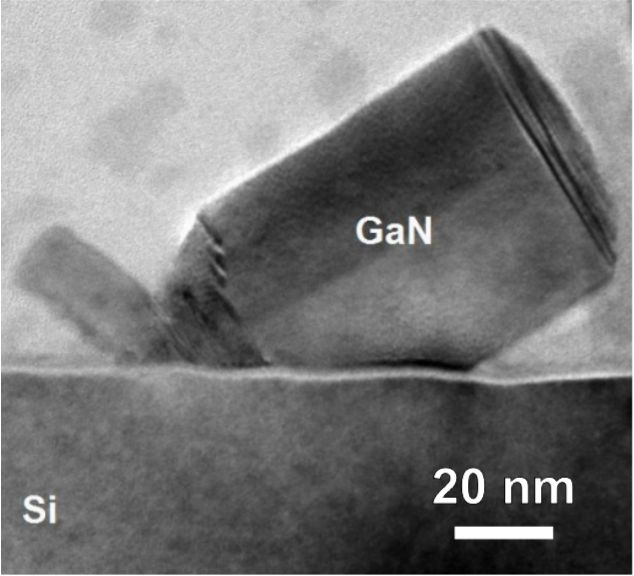
\includegraphics[height=0.2\textheight]{Image_16_1}}
	\end{minipage}
	\begin{minipage}[t]{0.25\linewidth}
		\center{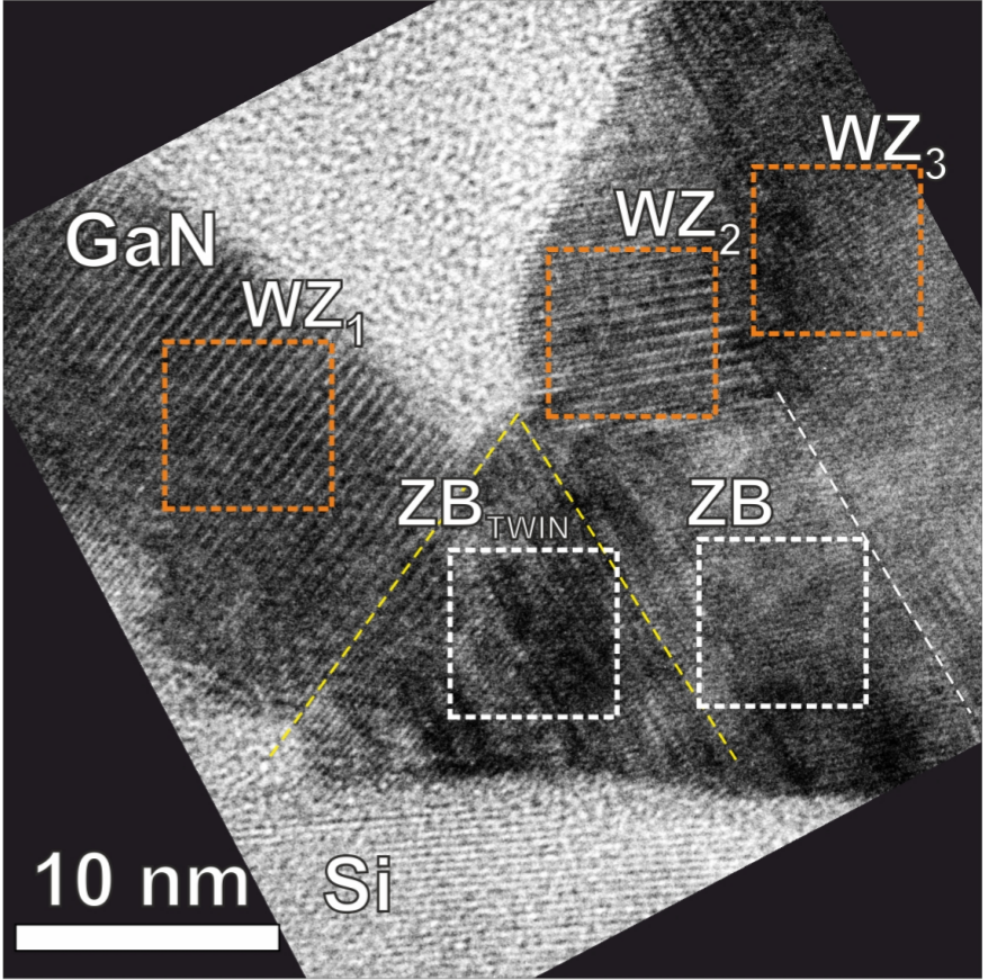
\includegraphics[height=0.2\textheight]{Image_16_2}}
	\end{minipage}
	\\
	\begin{minipage}[t]{0.15\linewidth}
		\center{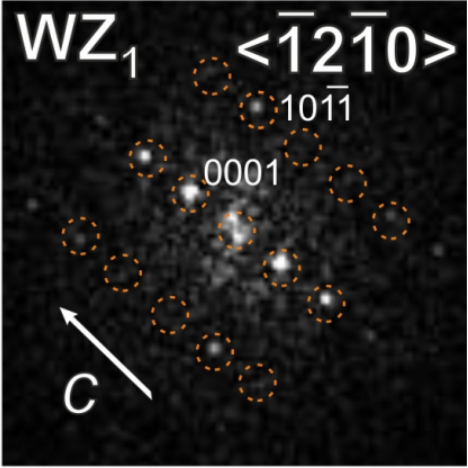
\includegraphics[height=0.15\textheight]{Image_16_3}}
	\end{minipage}
	\begin{minipage}[t]{0.15\linewidth}
		\center{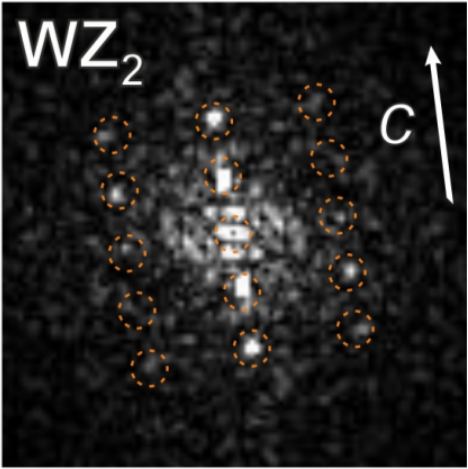
\includegraphics[height=0.15\textheight]{Image_16_4}}
	\end{minipage}
	\begin{minipage}[t]{0.15\linewidth}
		\center{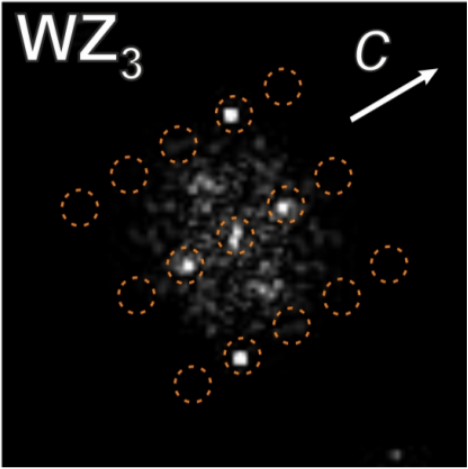
\includegraphics[height=0.15\textheight]{Image_16_5}}
	\end{minipage}
	\begin{minipage}[t]{0.15\linewidth}
		\center{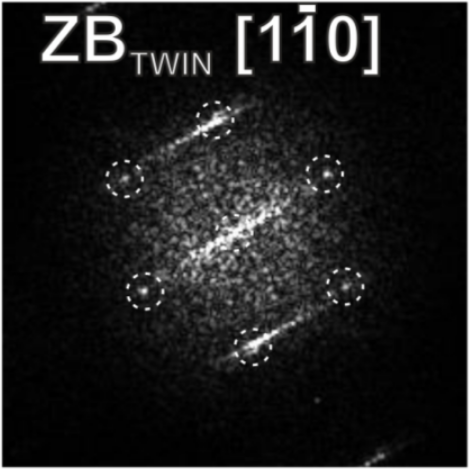
\includegraphics[height=0.15\textheight]{Image_16_6}}
	\end{minipage}
	\begin{minipage}[t]{0.15\linewidth}
		\center{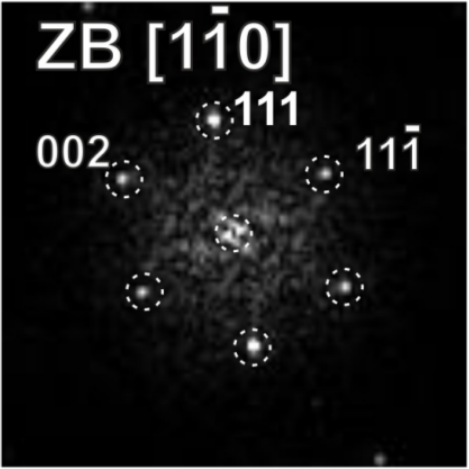
\includegraphics[height=0.15\textheight]{Image_16_7}}
	\end{minipage}
	\bigskip
	\hrule{}
	\bigskip
	\begin{minipage}[t]{0.25\linewidth}
		\center{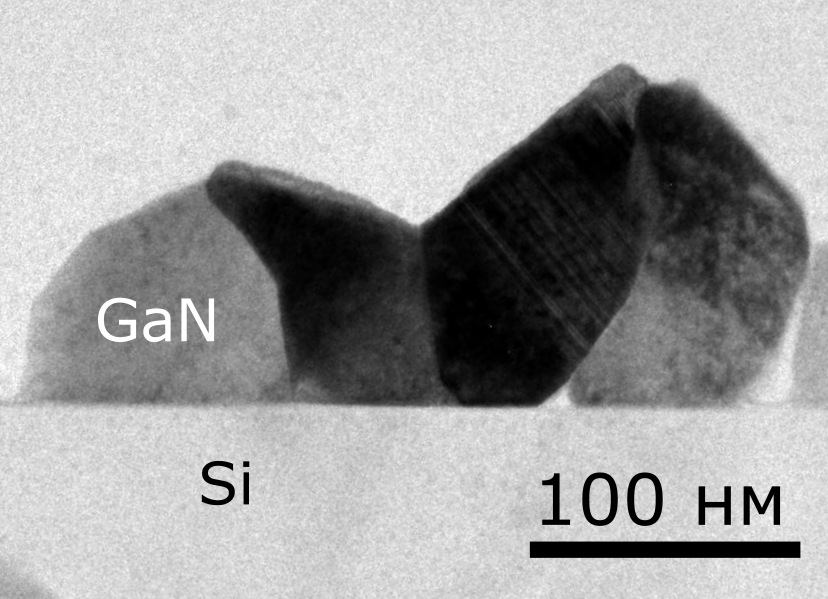
\includegraphics[height=0.2\textheight]{Image_18_1}}
	\end{minipage}
	\begin{minipage}[t]{0.25\linewidth}
		\center{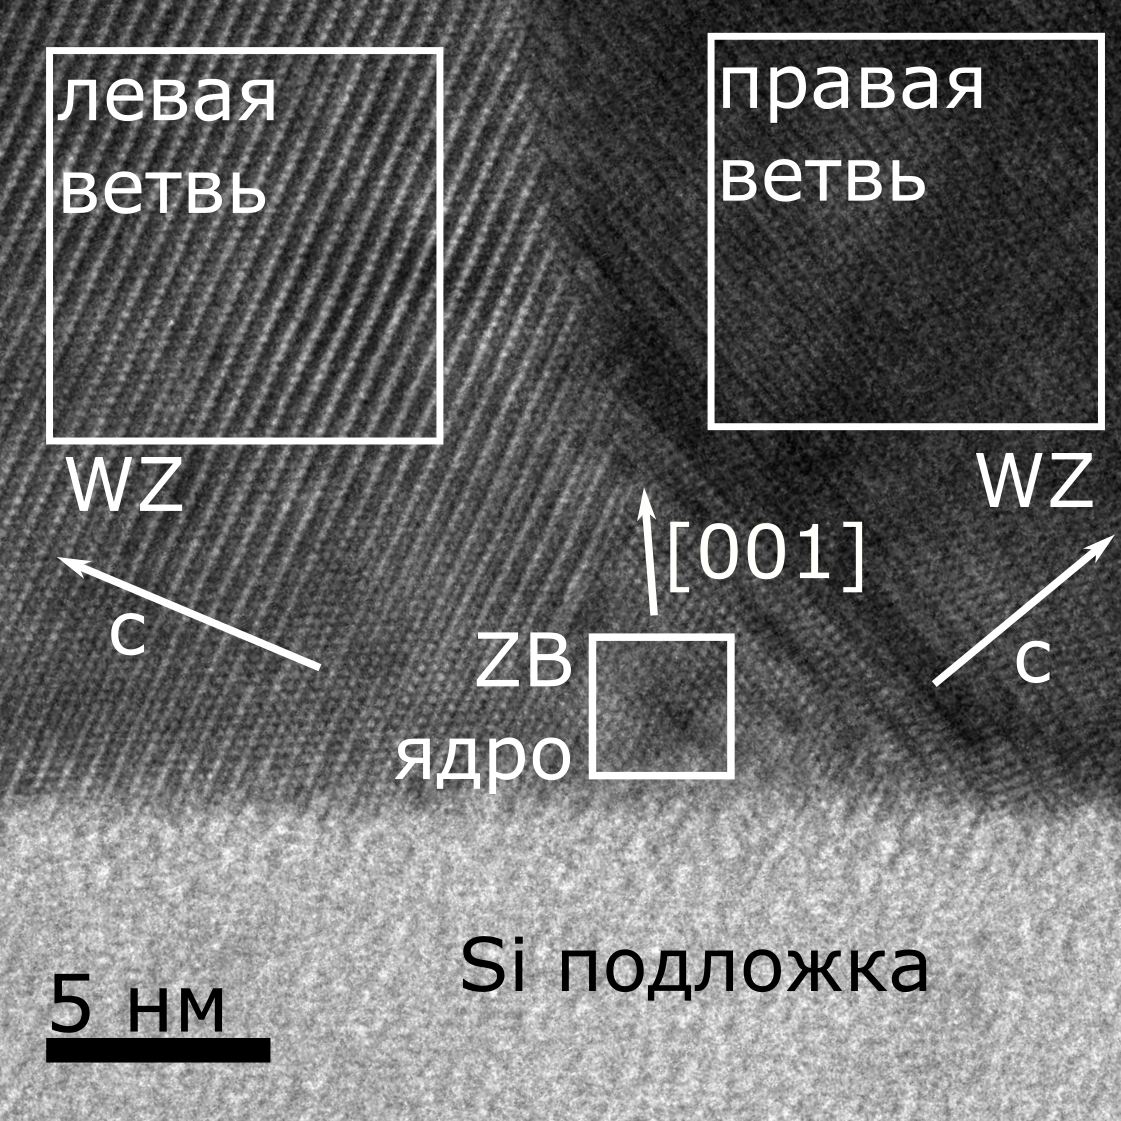
\includegraphics[height=0.2\textheight]{Image_18_2}}
	\end{minipage}
	\\
	\begin{minipage}[t]{0.2\linewidth}
		\center{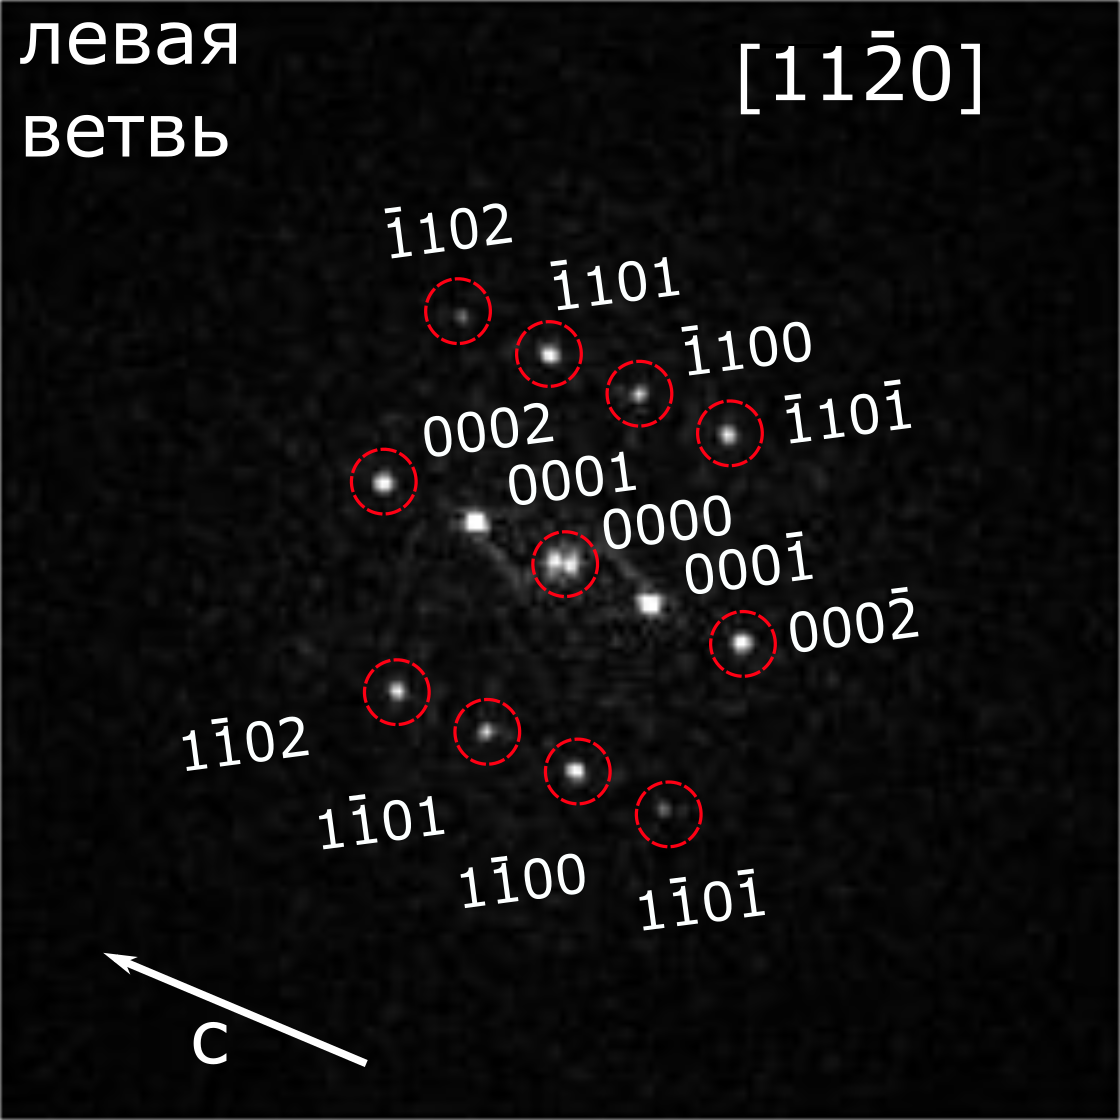
\includegraphics[height=0.2\textheight]{Image_18_3}}
	\end{minipage}
	\begin{minipage}[t]{0.2\linewidth}
		\center{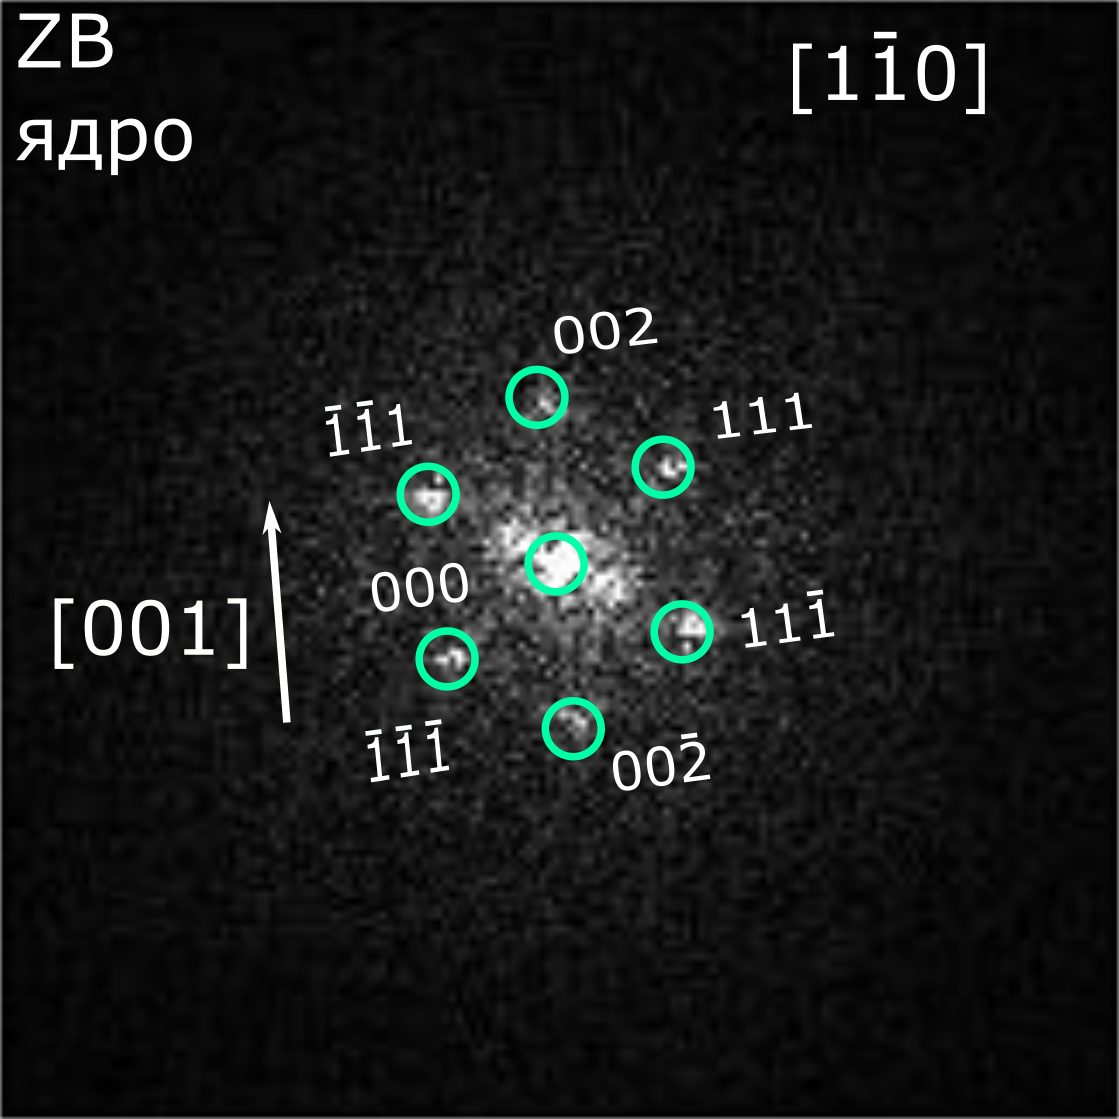
\includegraphics[height=0.2\textheight]{Image_18_4}}
	\end{minipage}
	\begin{minipage}[t]{0.2\linewidth}
		\center{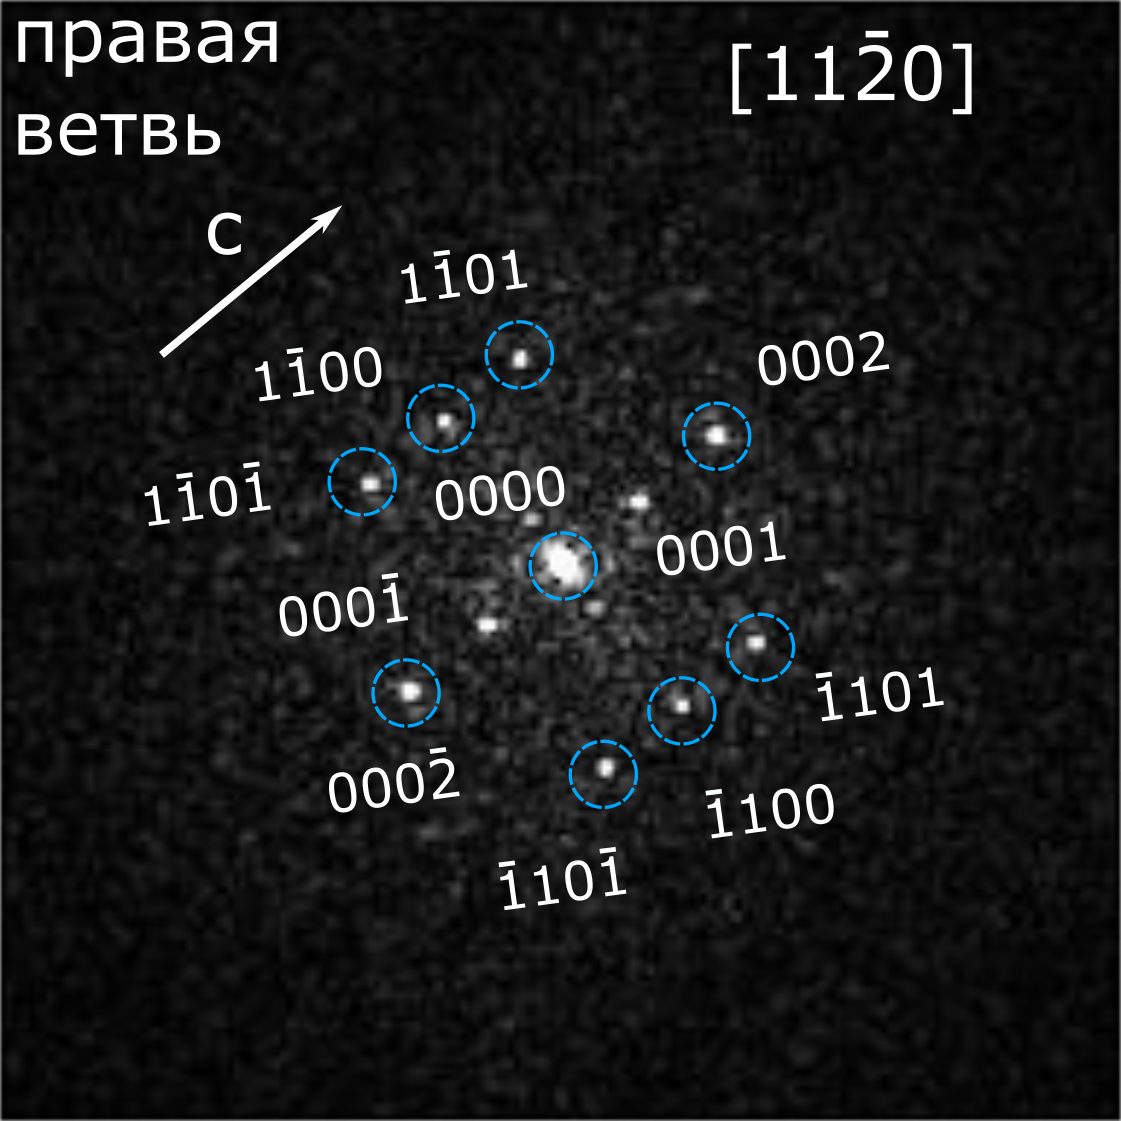
\includegraphics[height=0.2\textheight]{Image_18_5}}
	\end{minipage}
\end{frame}

\begin{frame}
	\frametitle{Фотолюминесценция GaN триподов}
	\centering
	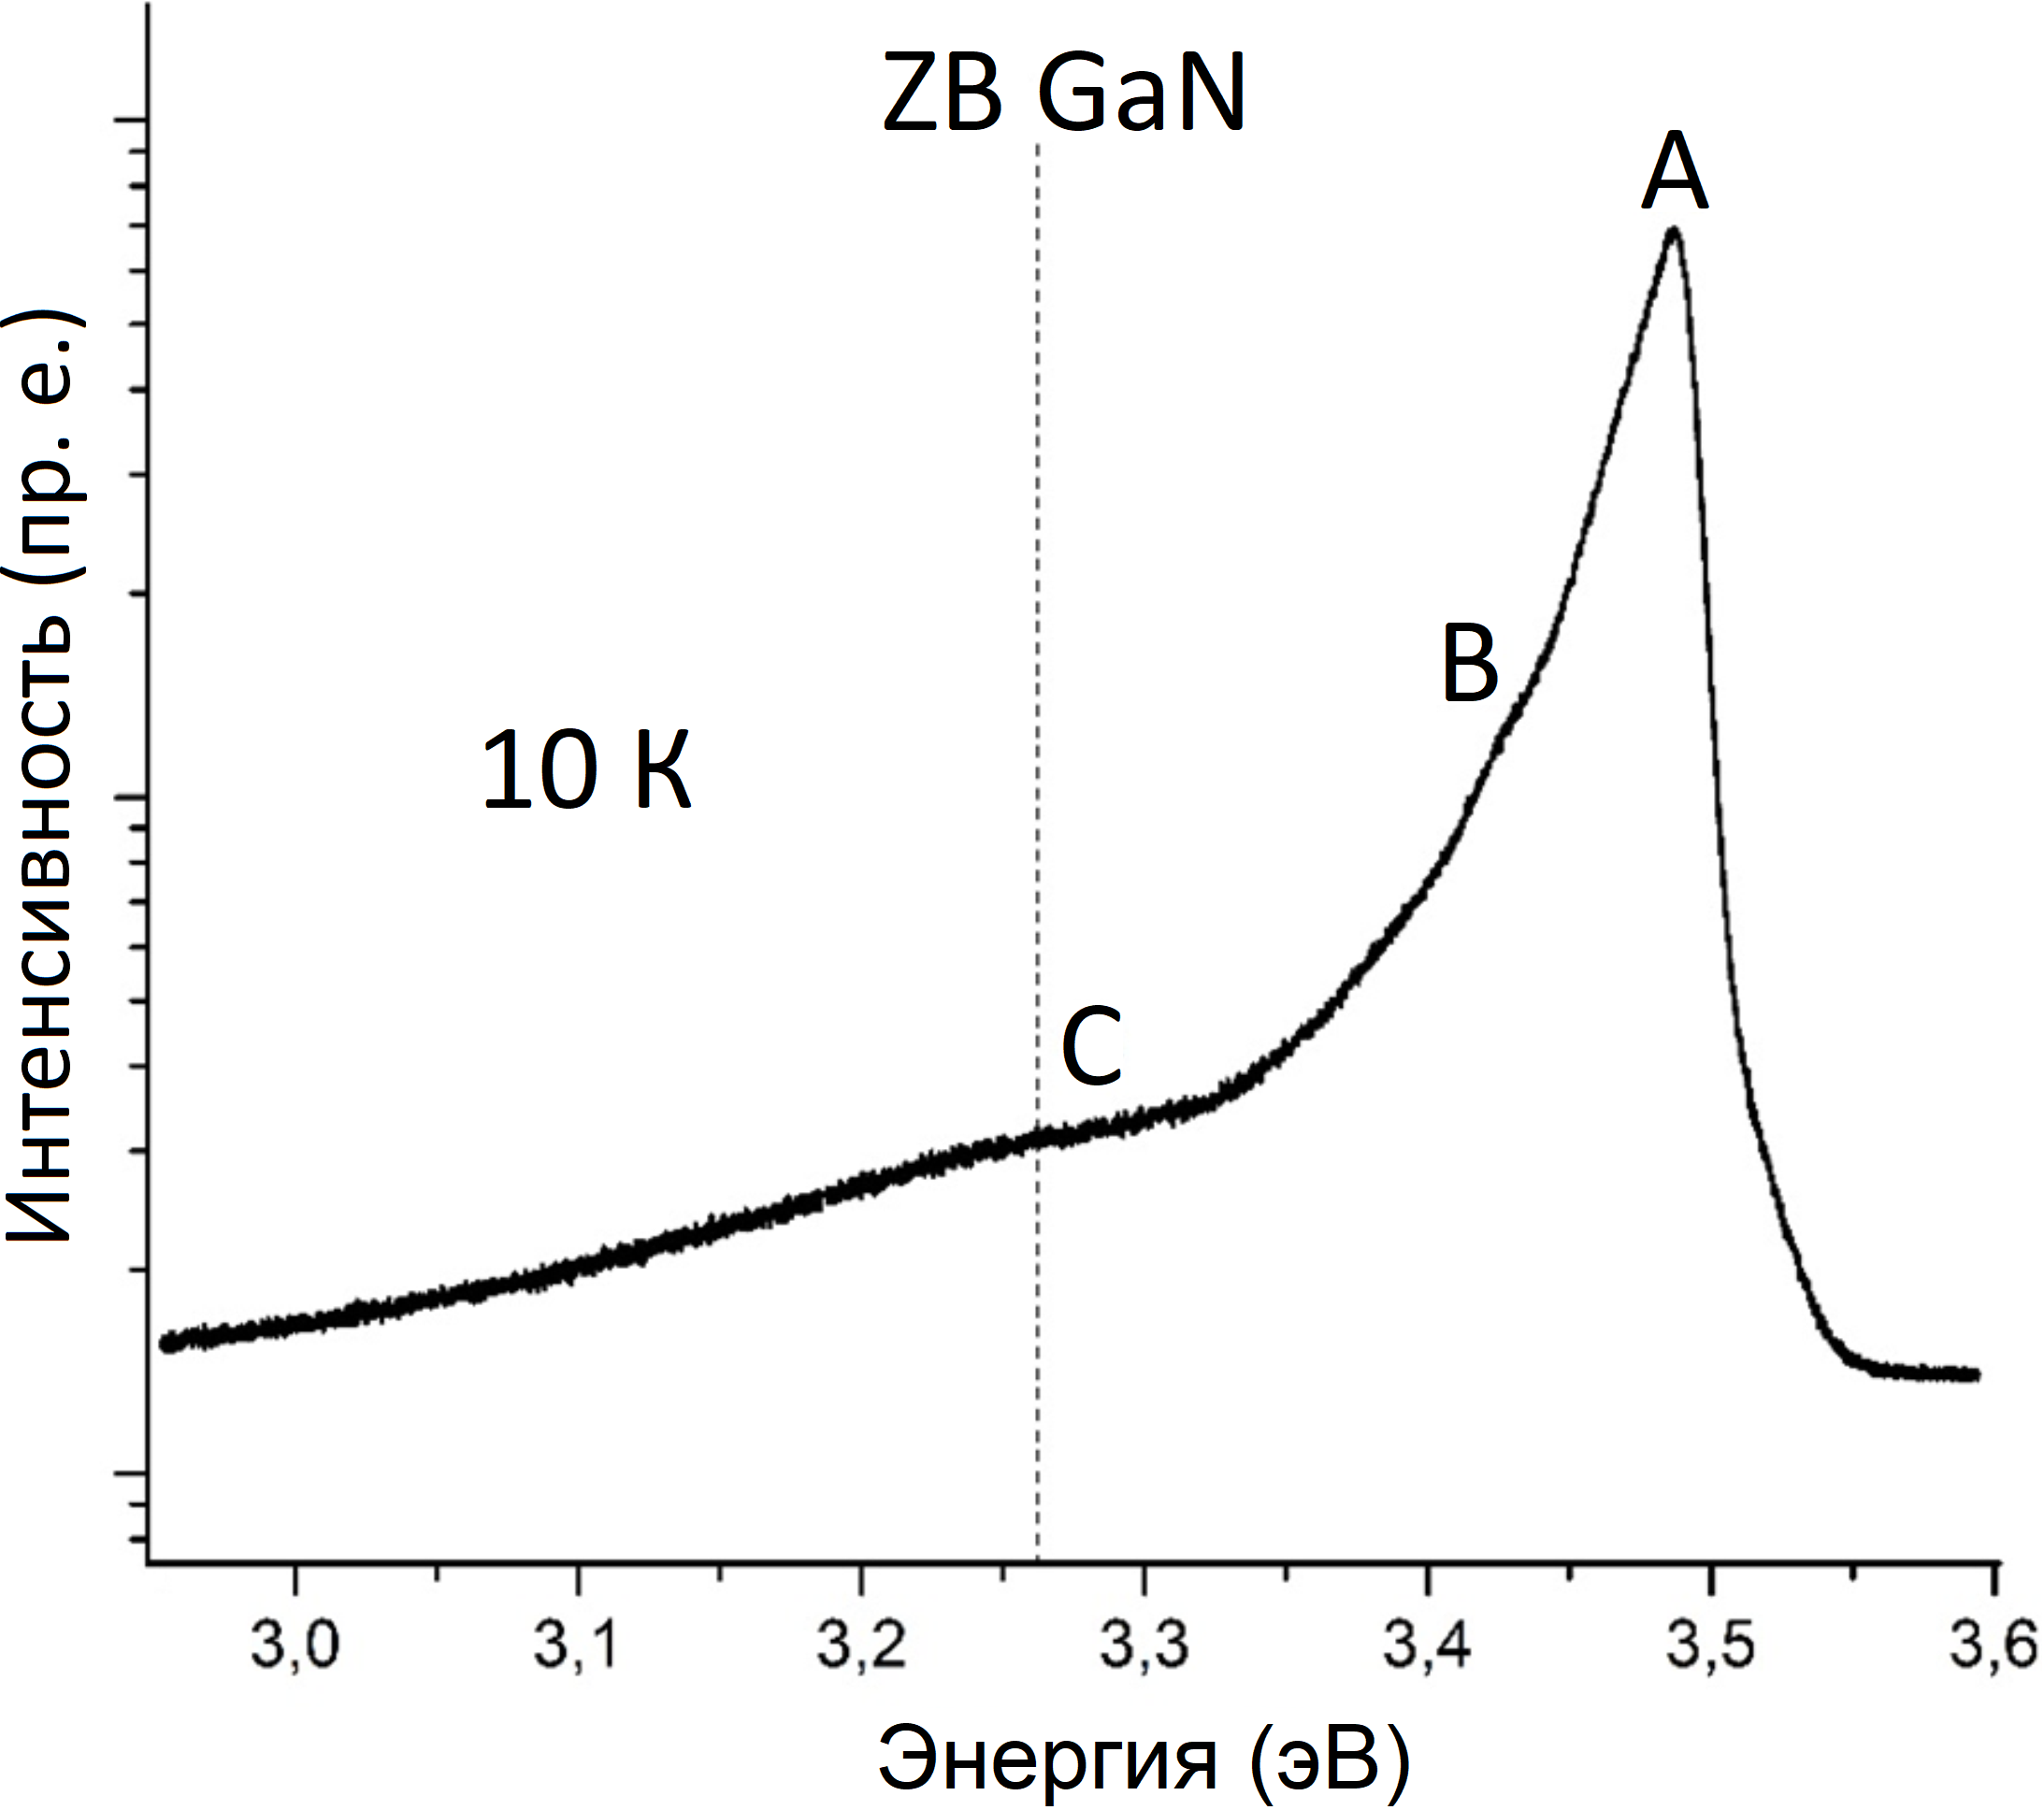
\includegraphics[width=0.6\linewidth]{Image_19}
\end{frame}

\begin{frame}[t]
	\frametitle{Влияние условий синтеза на морфологию GaN наноструктур}
	\centering
	\begin{minipage}[t]{0.9\linewidth}
		\begin{columns}[onlytextwidth]
			\begin{column}{0.4\textwidth}
				\centering
				\text{Нитридация}
				\\
				\begin{minipage}[t]{0.45\linewidth}
					\center{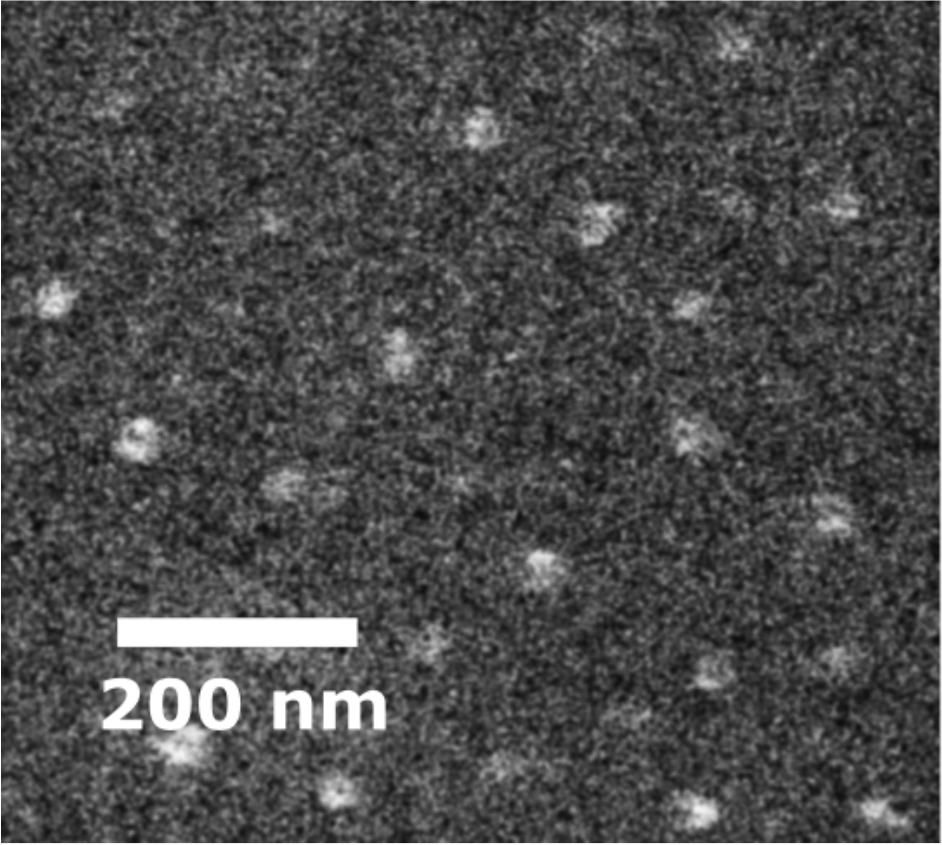
\includegraphics[height=0.21\textheight]{Image_20_1}}
				\end{minipage}
				\begin{minipage}[t]{0.45\linewidth}
					\center{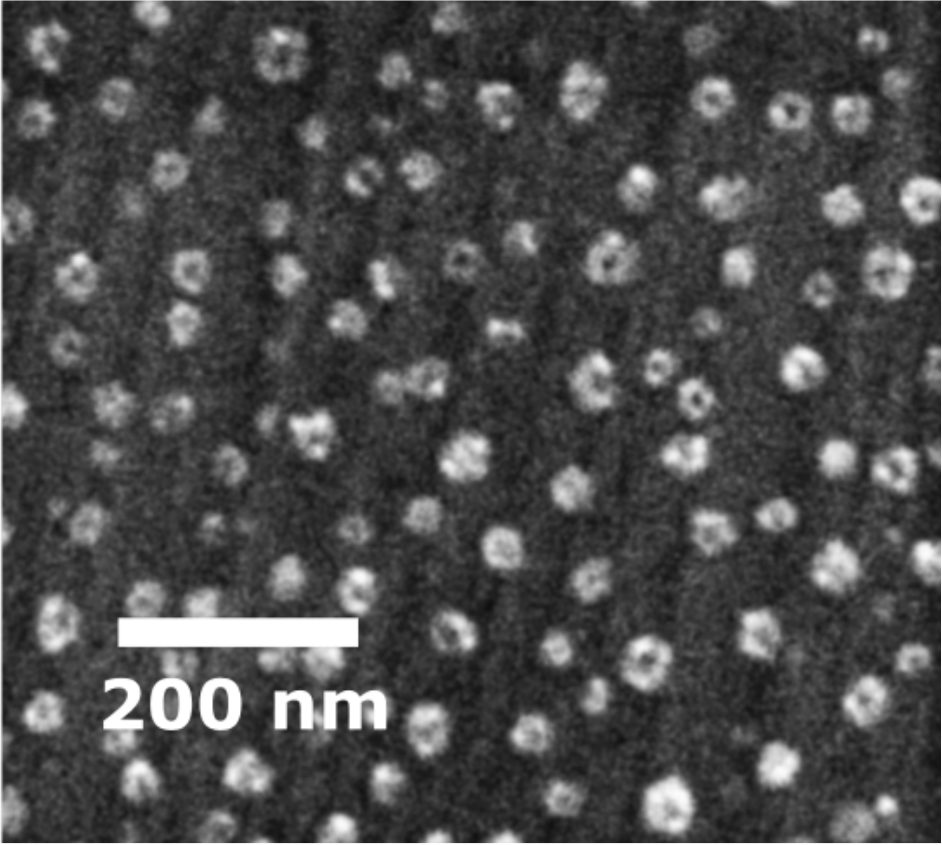
\includegraphics[height=0.21\textheight]{Image_20_2}}
				\end{minipage}
			\end{column}
			\begin{column}{0.55\textwidth}
				\centering
				\text{Поток Ga}
				\\
				\begin{minipage}[t]{0.3\linewidth}
					\center{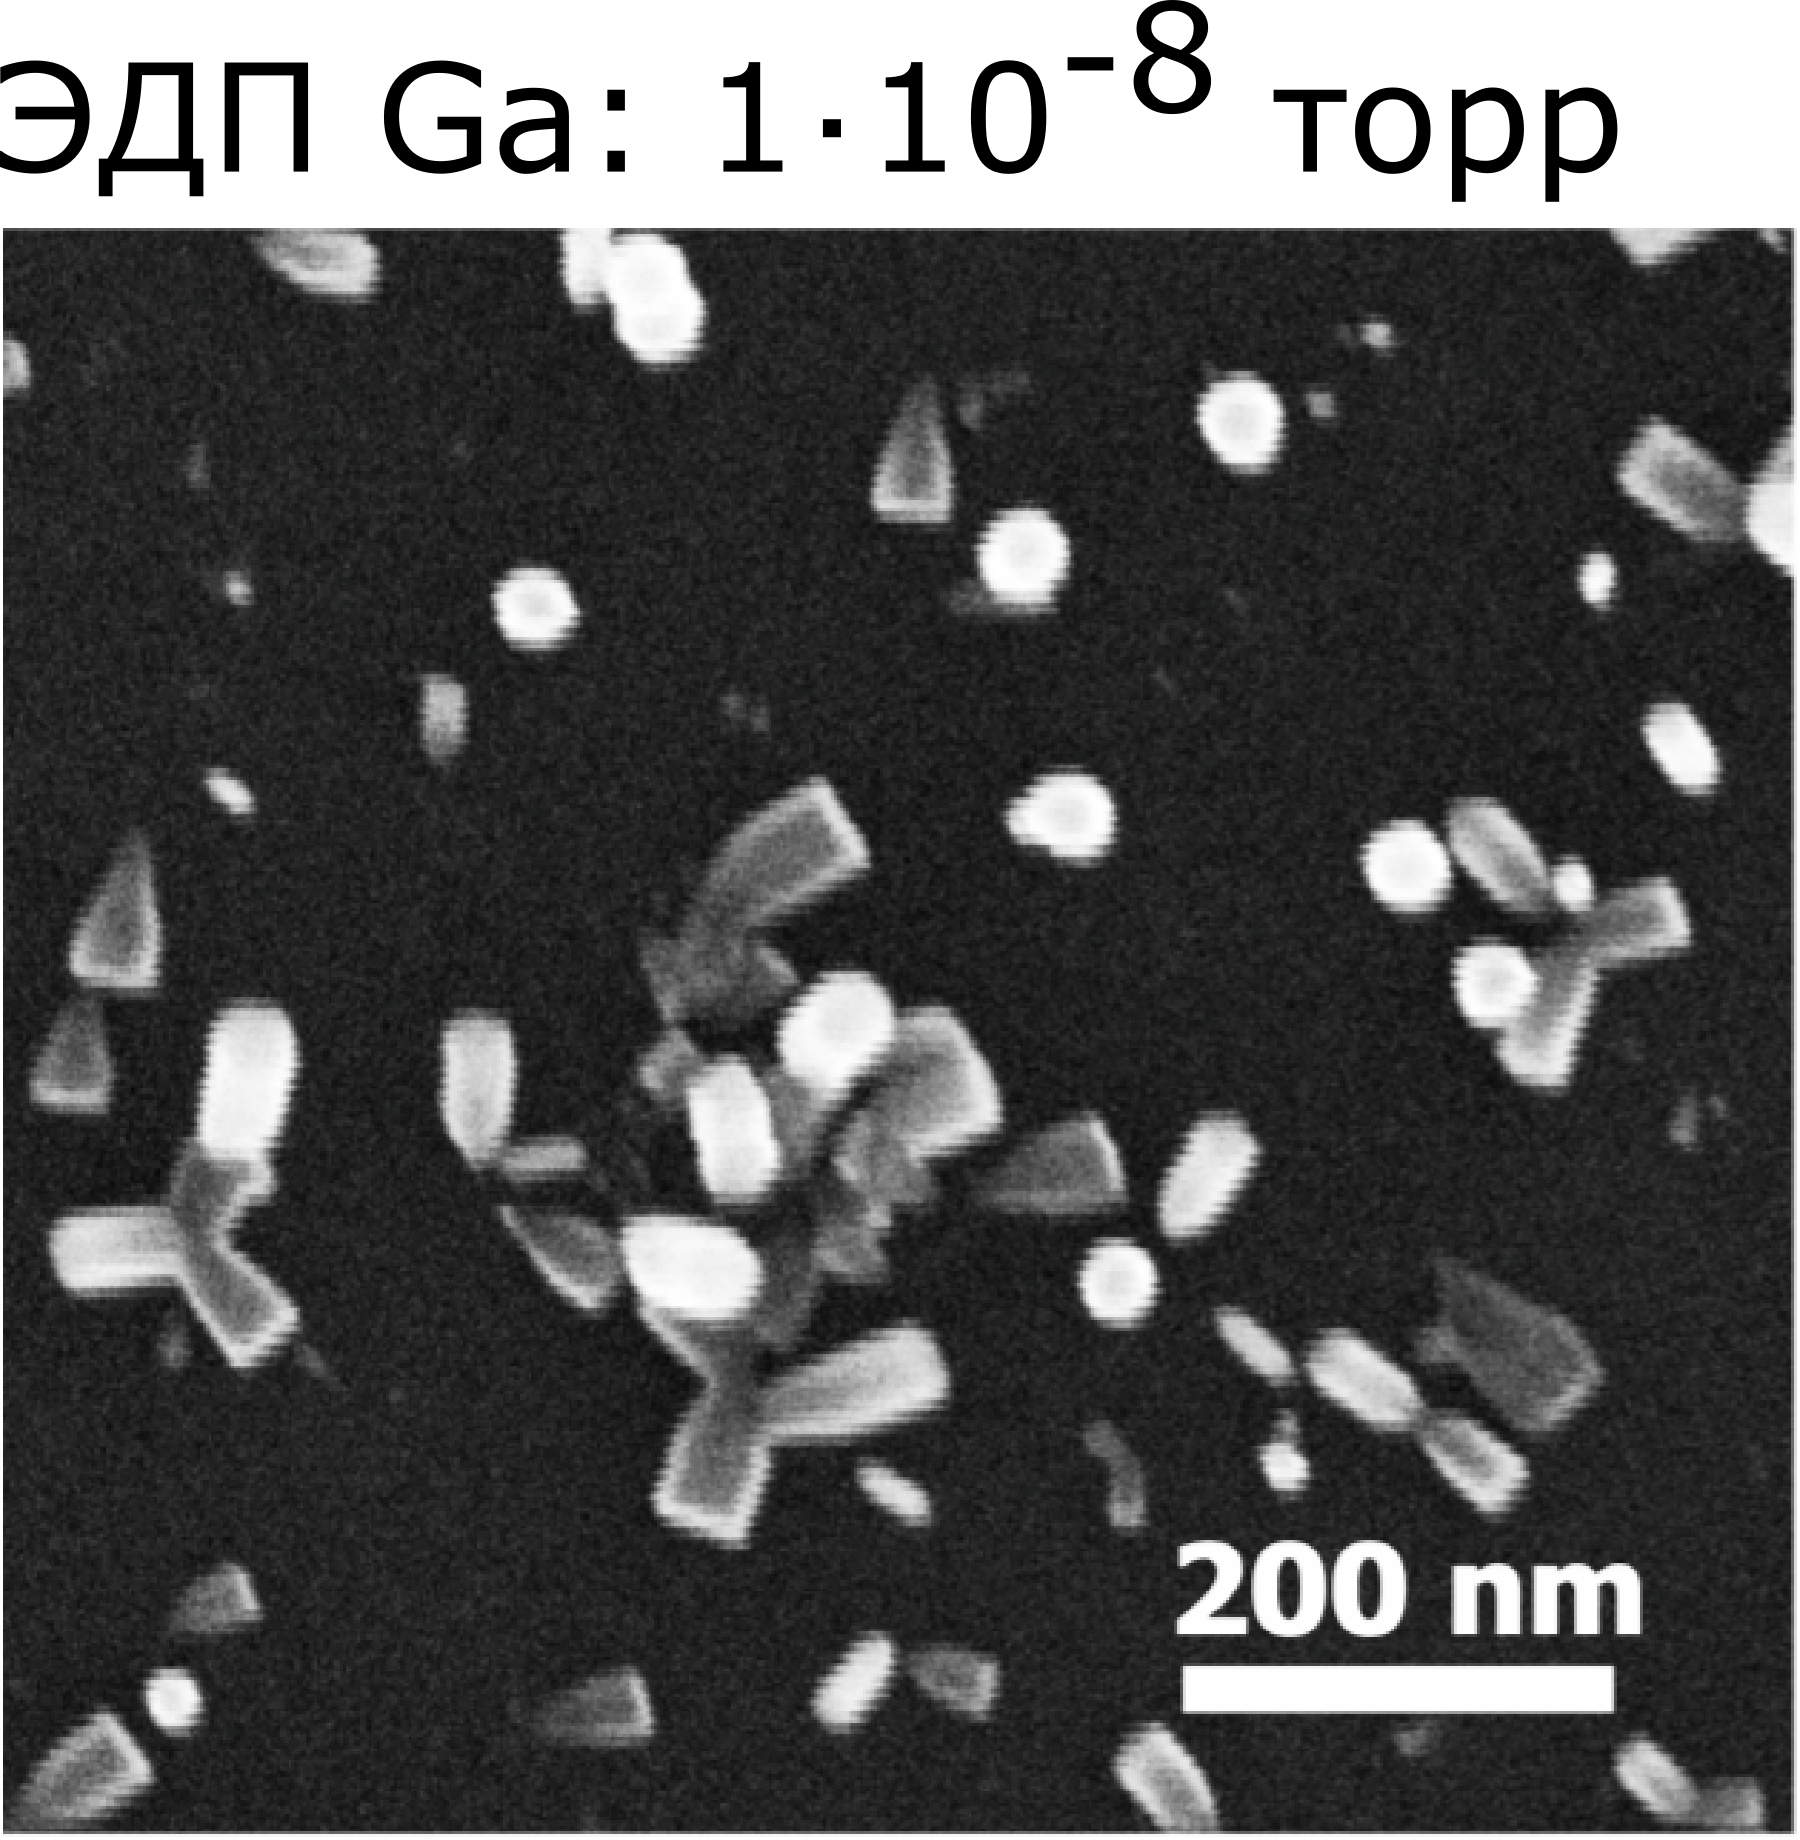
\includegraphics[height=0.21\textheight]{Image_23_1}}
				\end{minipage}
				\begin{minipage}[t]{0.3\linewidth}
					\center{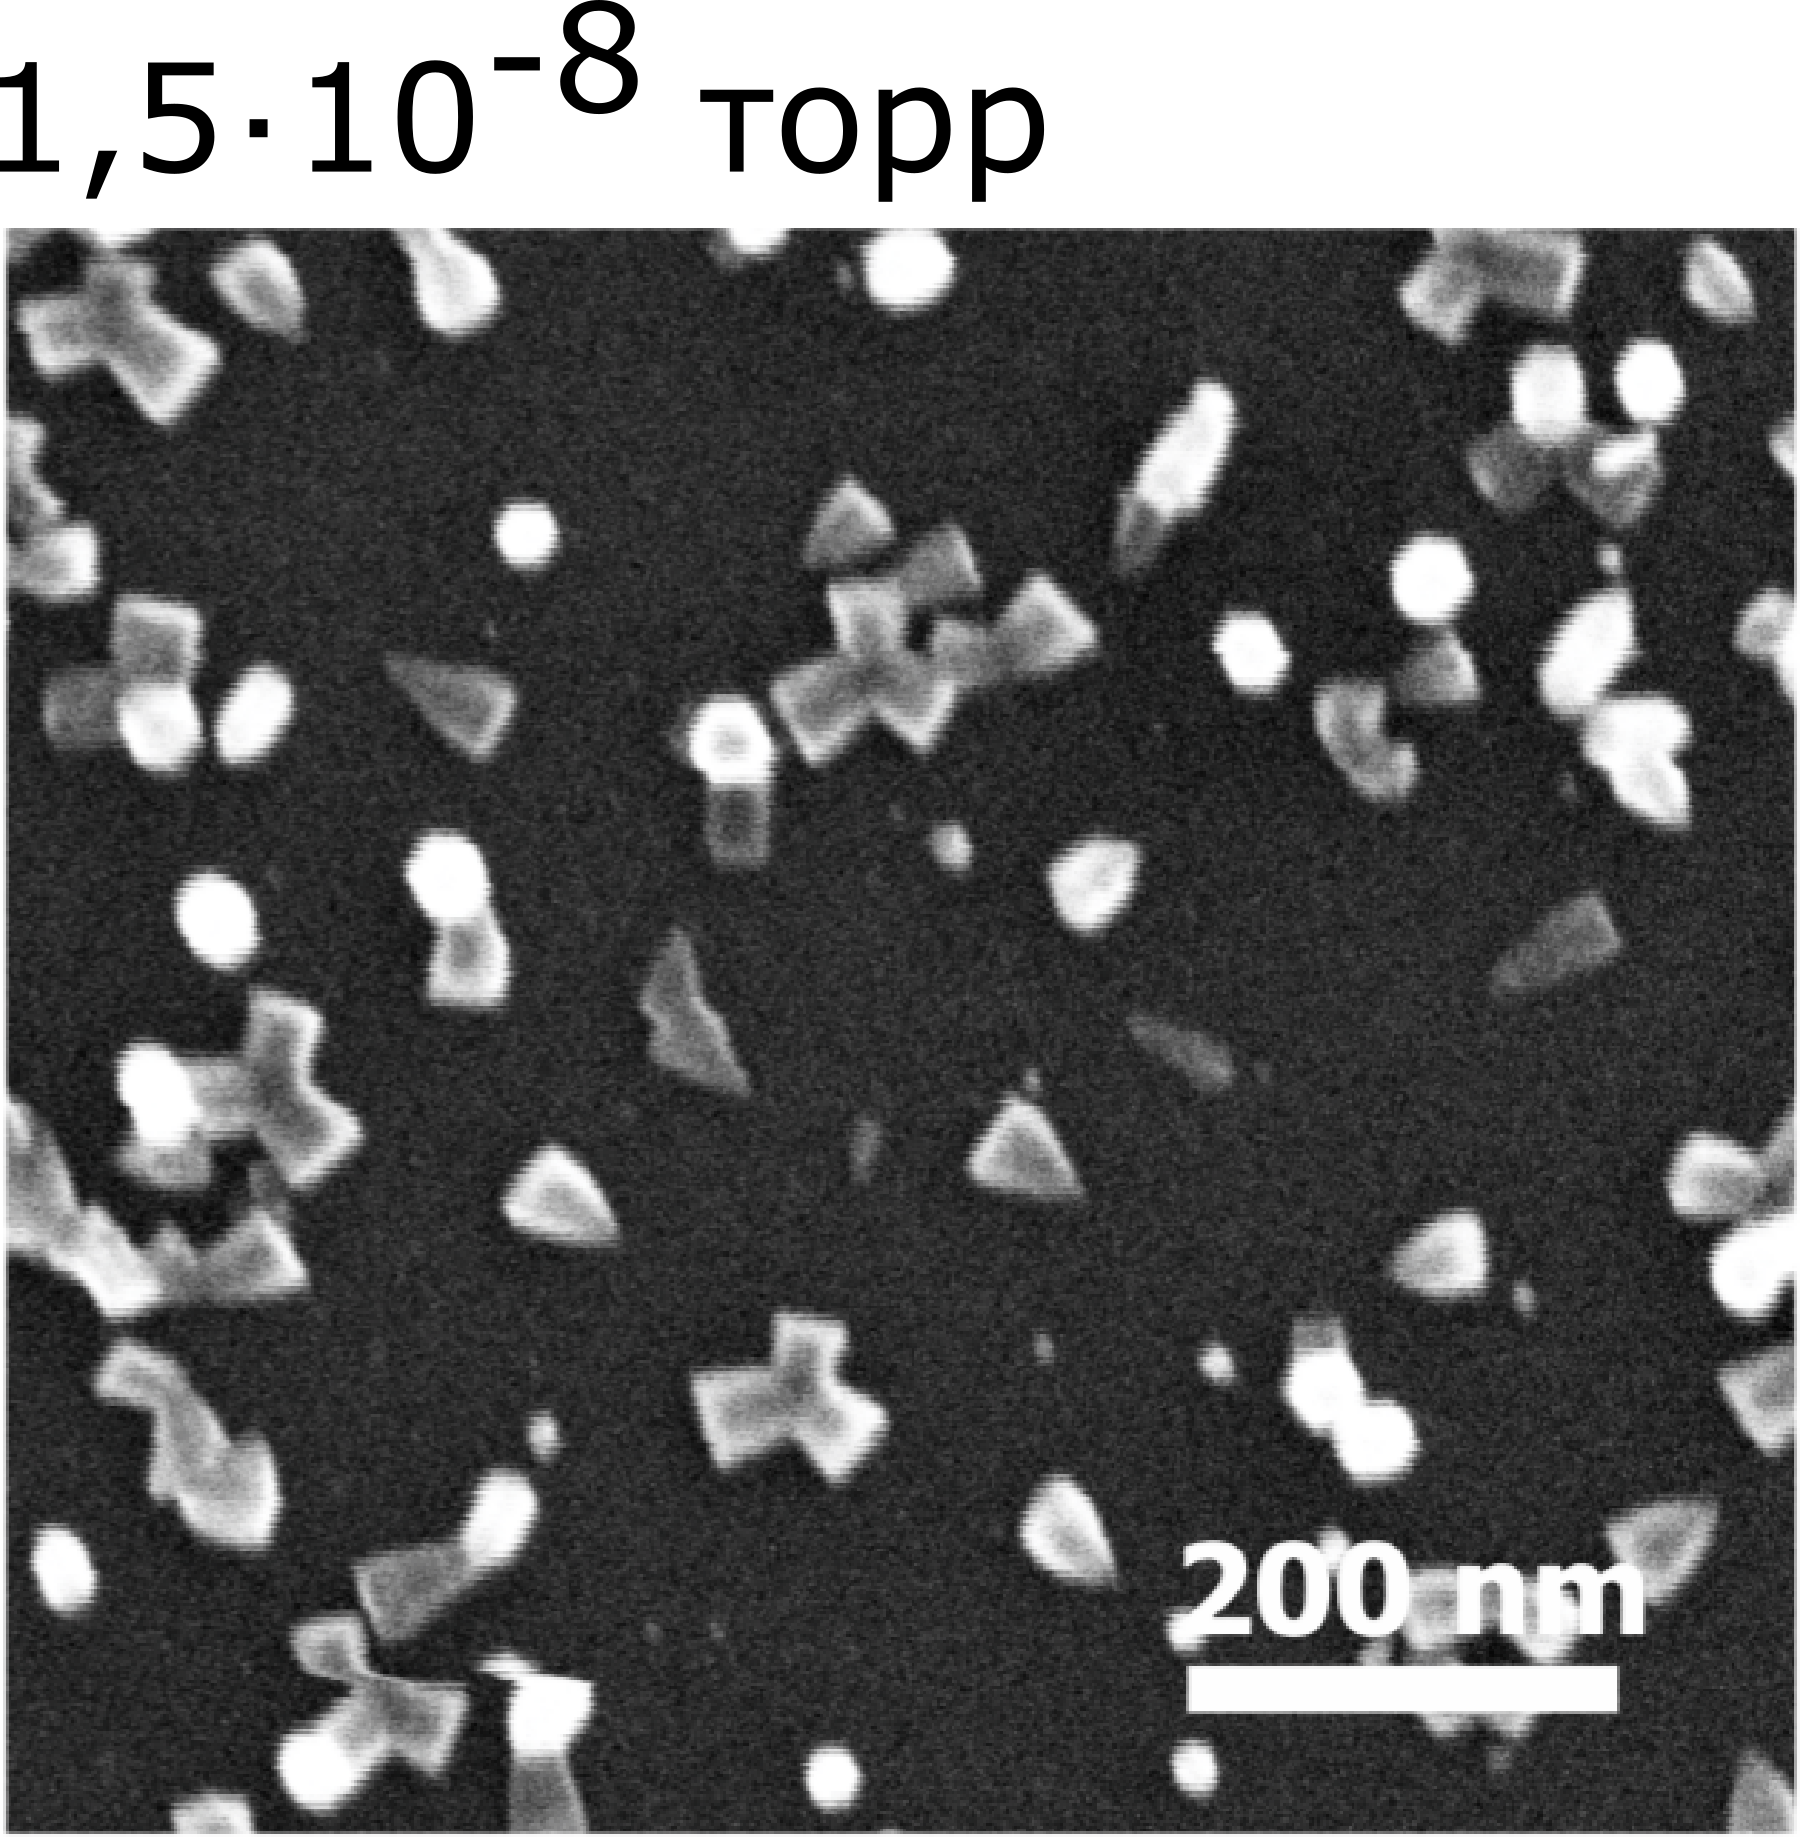
\includegraphics[height=0.21\textheight]{Image_23_2}}
				\end{minipage}
				\begin{minipage}[t]{0.3\linewidth}
					\center{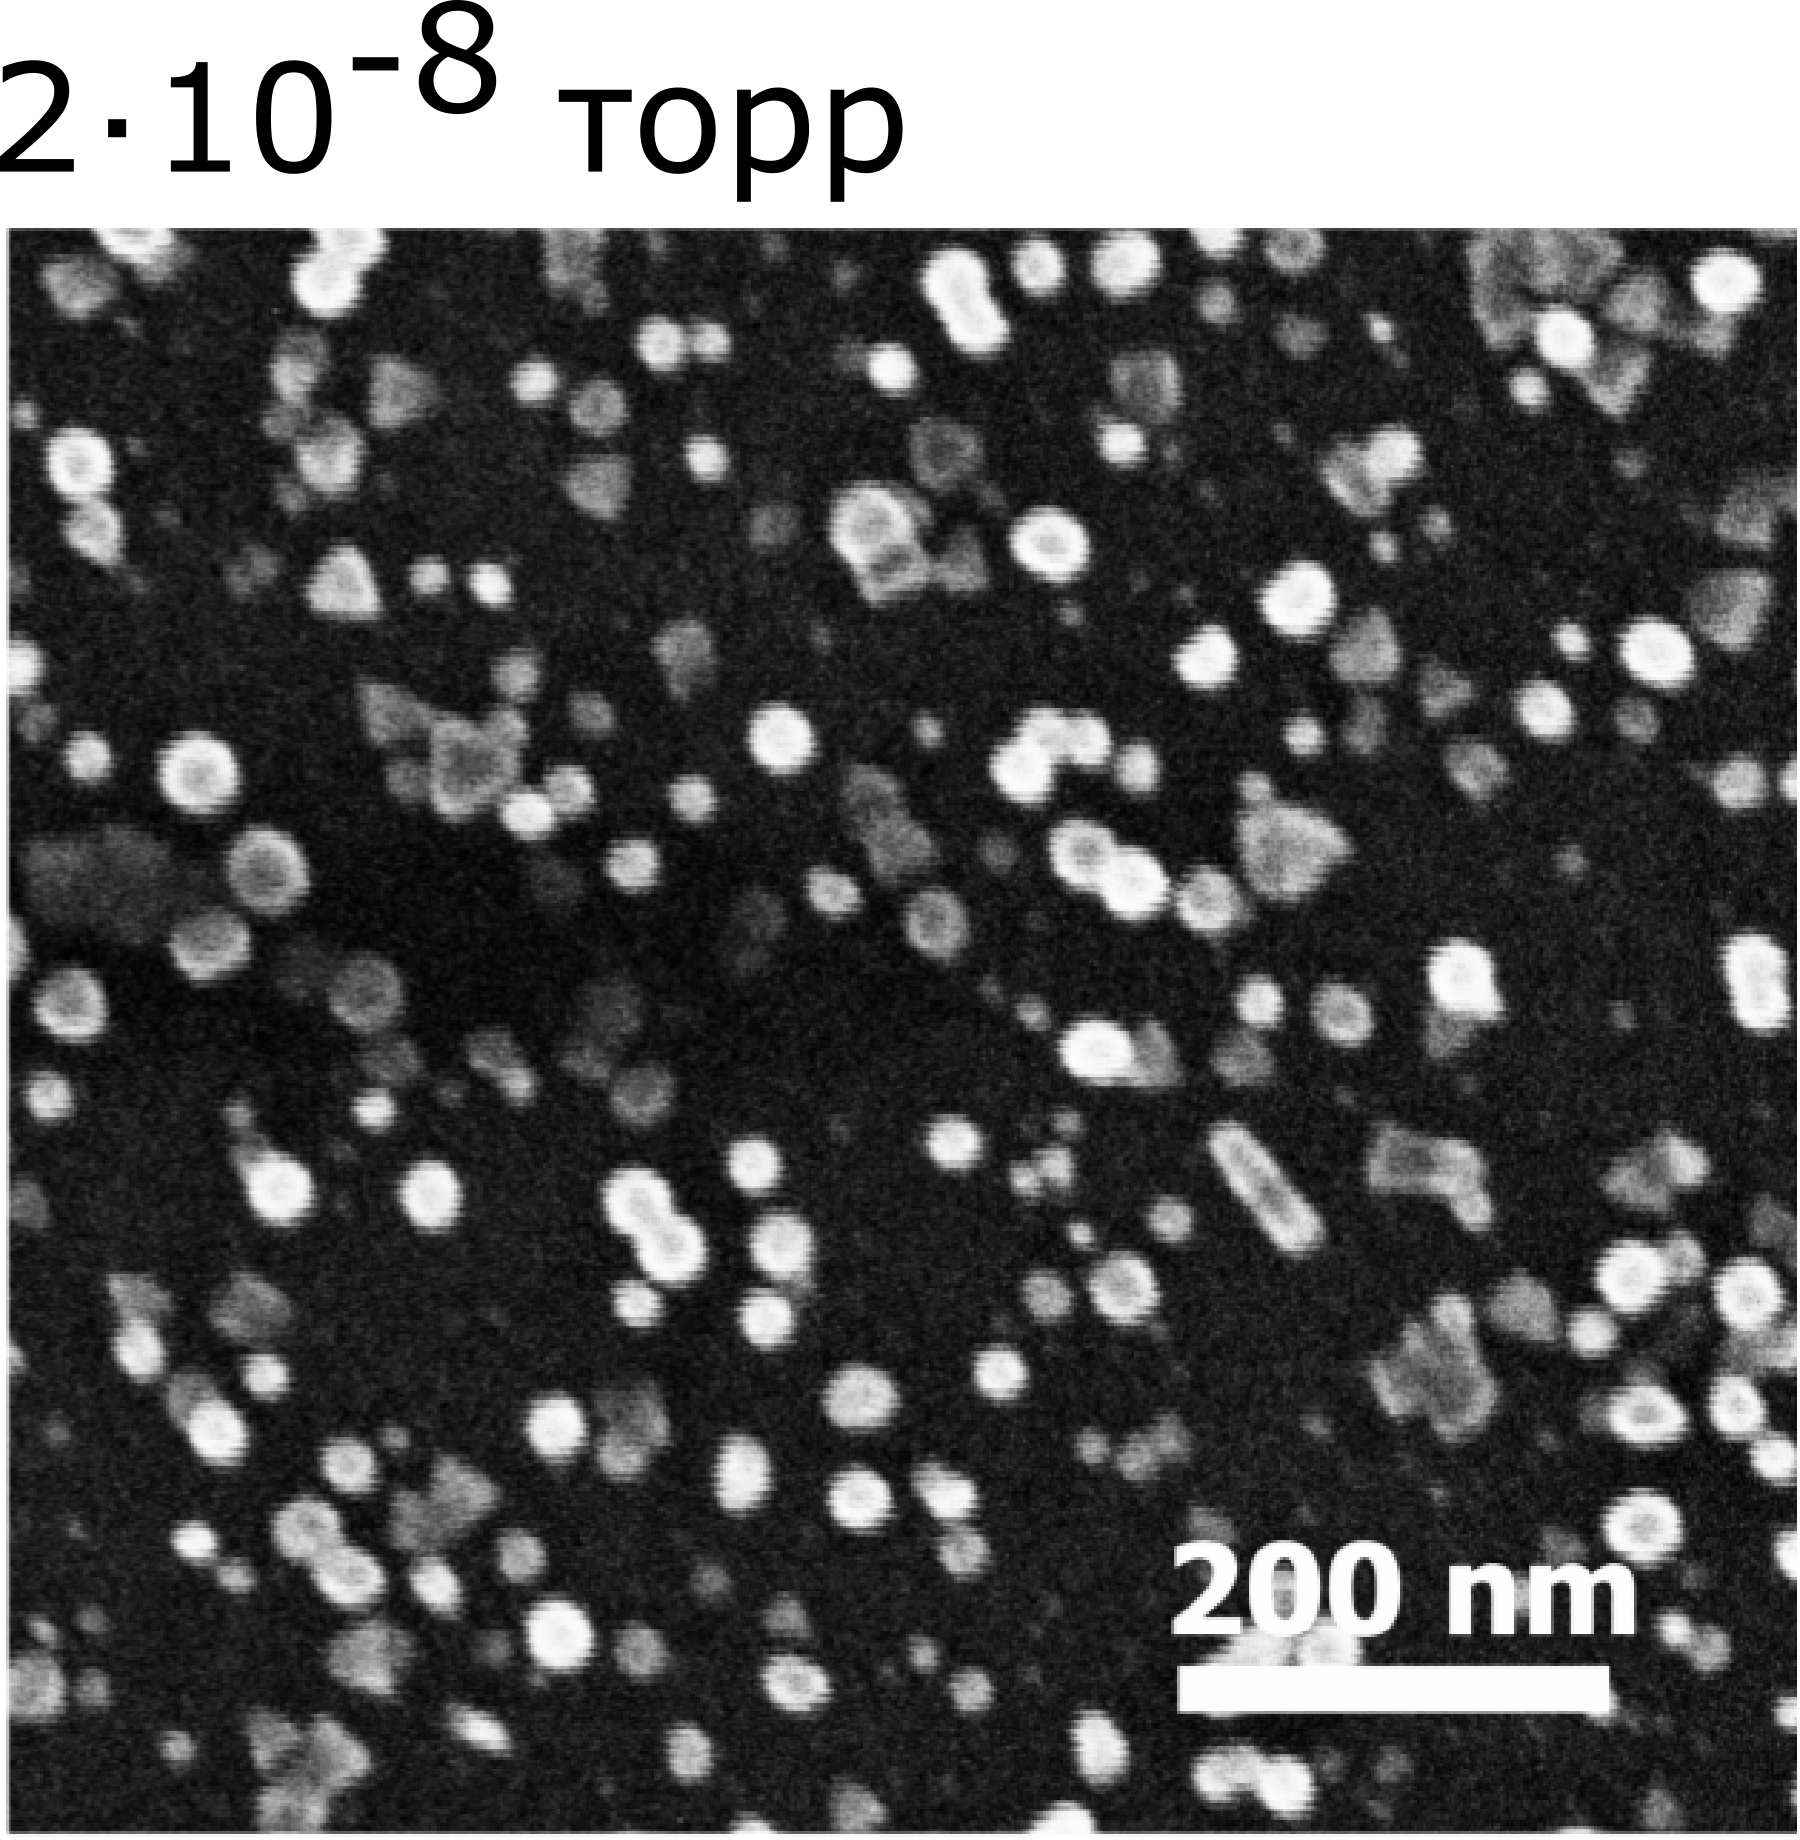
\includegraphics[height=0.21\textheight]{Image_23_3}}
				\end{minipage}
			\end{column}
		\end{columns}
	\end{minipage}
	\\[15pt]
	\begin{minipage}[t]{0.9\linewidth}
		\begin{columns}[onlytextwidth]
			\begin{column}{0.4\textwidth}
				\centering
				\text{Рост}
				\\
				\begin{minipage}[t]{0.45\linewidth}
					\center{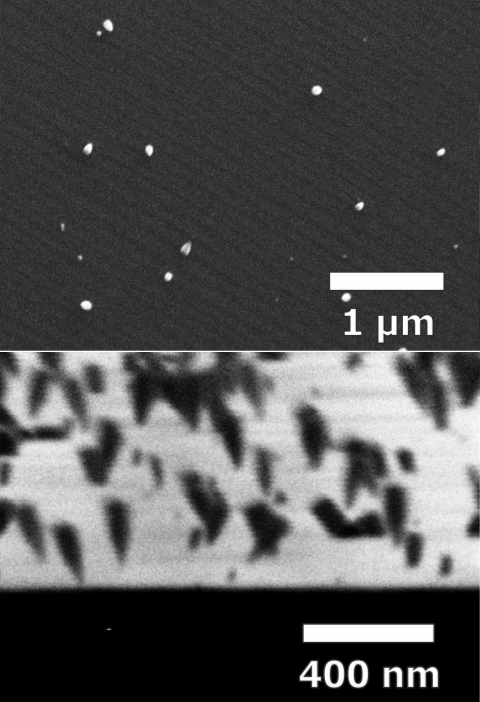
\includegraphics[height=0.33\textheight]{Image_21_1}}
				\end{minipage}
				\begin{minipage}[t]{0.45\linewidth}
					\center{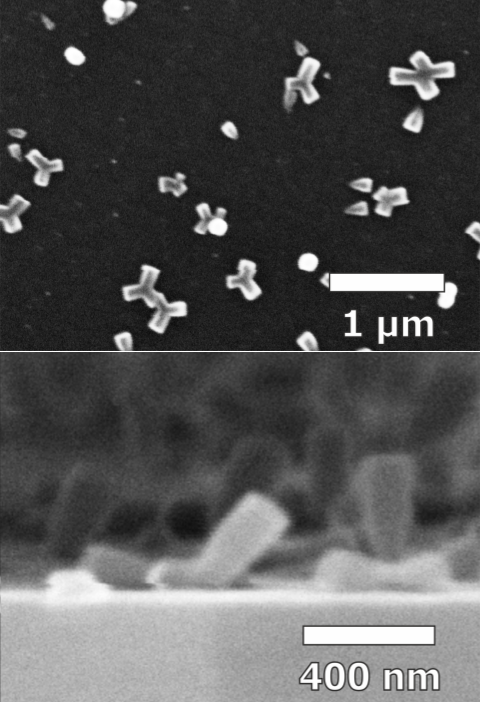
\includegraphics[height=0.33\textheight]{Image_21_2}}
				\end{minipage}
			\end{column}
			\begin{column}{0.55\textwidth}
				\centering
				\text{Температура роста}
				\\
				\begin{minipage}[t]{0.3\linewidth}
					\center{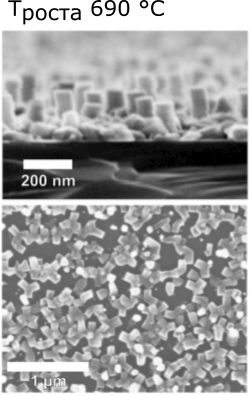
\includegraphics[height=0.33\textheight]{Image_25_1}}
				\end{minipage}
				\begin{minipage}[t]{0.3\linewidth}
					\center{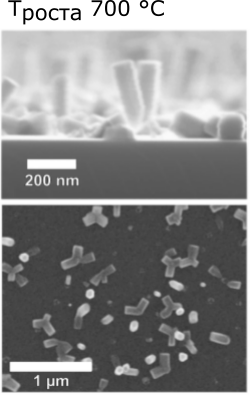
\includegraphics[height=0.33\textheight]{Image_25_2}}
				\end{minipage}
				\begin{minipage}[t]{0.3\linewidth}
					\center{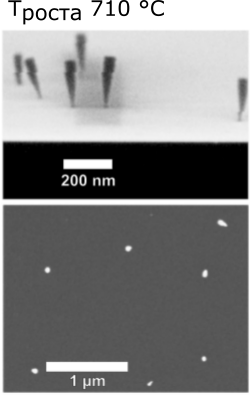
\includegraphics[height=0.33\textheight]{Image_25_3}}
				\end{minipage}
			\end{column}
		\end{columns}
	\end{minipage}
\end{frame}

\begin{frame}
	\frametitle{Положение №1}
	\large
	Установлено, что в процессе капельной молекулярно-пучковой эпитаксии на
	поверхности Si(111) могут формироваться GaN наноостровки с метастабильной
	структурой сфалерита. При последующем росте GaN
	% в условиях пониженной температуры (\(\approx 690\)~\si{\degreeCelsius}) и
	% пониженного потока Ga (\(\approx 1 \cdot 10^{-8}\)~\si{\torr})
	на \{111\} гранях наноостровков могут зарождаться наклонные наноколонны со
	структурой вюрцита, что приводит к формированию наноструктур в форме
	трипода.
\end{frame}

\begin{frame}
	\frametitle{Влияние подготовки поверхности на морфологию GaN ННК}
	\centering
	\begin{minipage}[t]{0.31\linewidth}
		\center{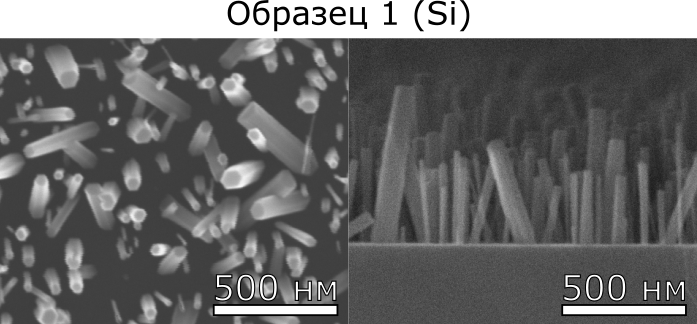
\includegraphics[width=1\linewidth]{Image_27_1}}
	\end{minipage}
	\\
	\bigskip
	\begin{minipage}[t]{0.31\linewidth}
		\center{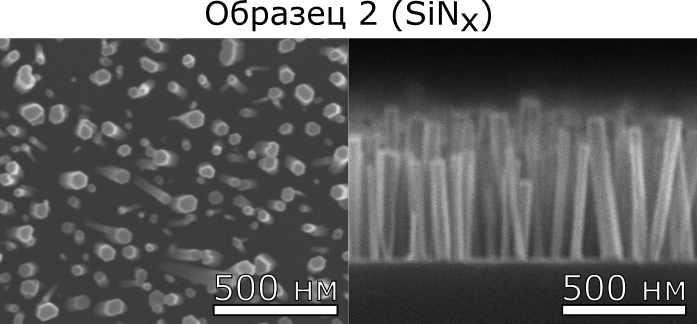
\includegraphics[width=1\linewidth]{Image_27_2}}
	\end{minipage}
	\begin{minipage}[t]{0.31\linewidth}
		\center{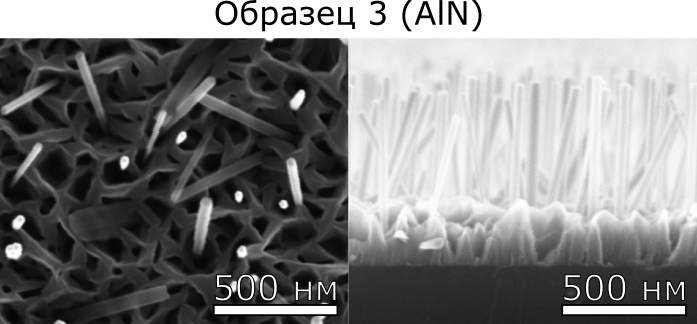
\includegraphics[width=1\linewidth]{Image_27_3}}
	\end{minipage}
	\begin{minipage}[t]{0.31\linewidth}
		\center{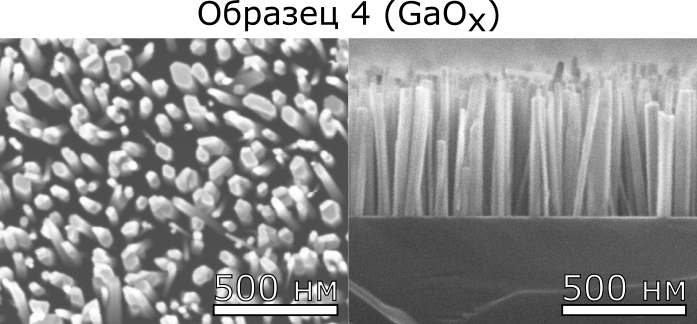
\includegraphics[width=1\linewidth]{Image_27_4}}
	\end{minipage}
	\\
	\bigskip
	\begin{minipage}[t]{0.31\linewidth}
		\center{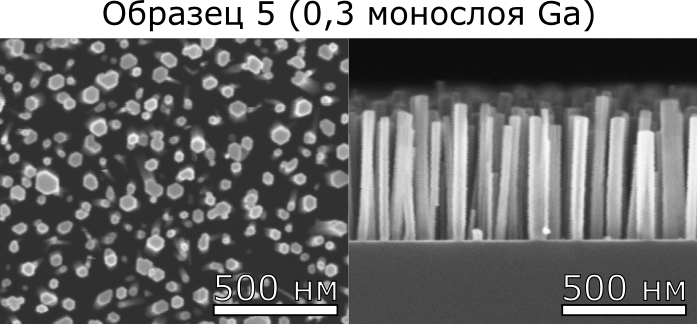
\includegraphics[width=1\linewidth]{Image_27_5}}
	\end{minipage}
	\begin{minipage}[t]{0.31\linewidth}
		\center{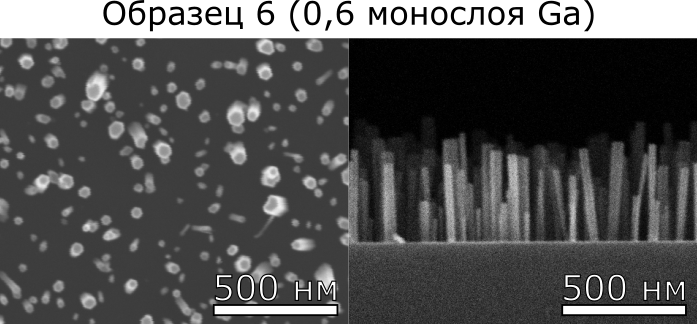
\includegraphics[width=1\linewidth]{Image_27_6}}
	\end{minipage}
	\begin{minipage}[t]{0.31\linewidth}
		\center{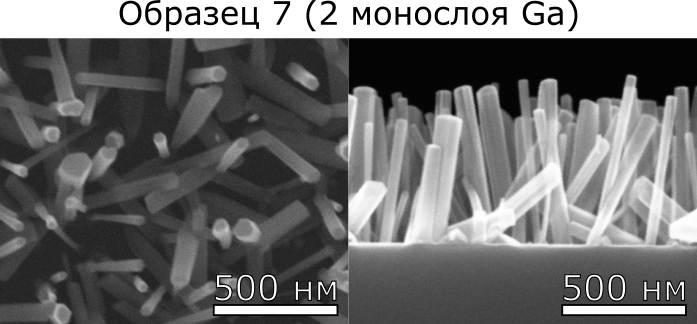
\includegraphics[width=1\linewidth]{Image_27_7}}
	\end{minipage}
\end{frame}

\begin{frame}
	\frametitle{Влияние подготовки поверхности на морфологию GaN ННК}
	\centering
	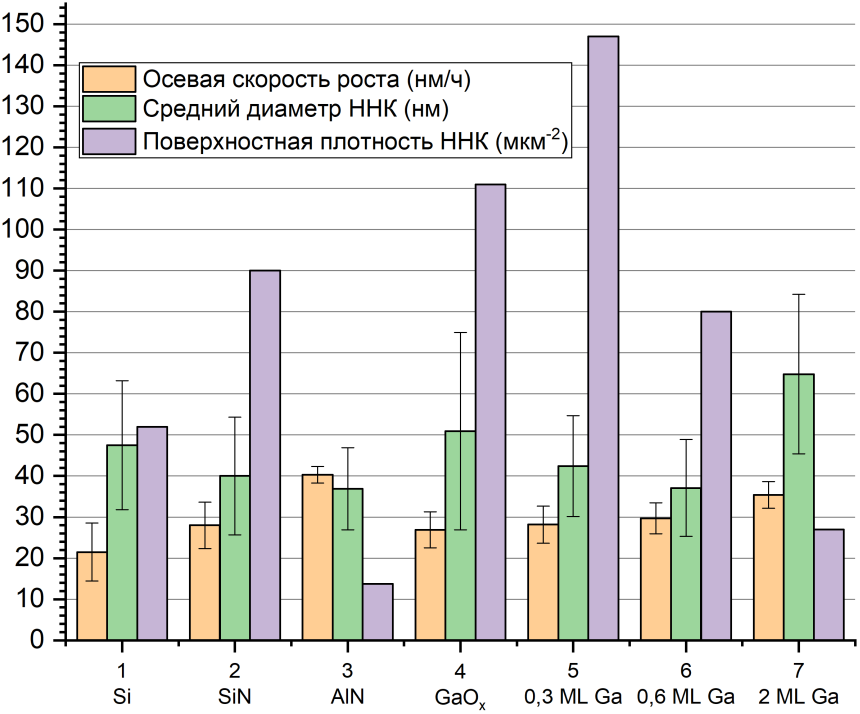
\includegraphics[width=0.7\linewidth]{Image_28}
\end{frame}

\begin{frame}
	\frametitle{Влияние подготовки поверхности на ФЛ GaN ННК}
	\centering
	\begin{minipage}[t]{0.47\linewidth}
		\center{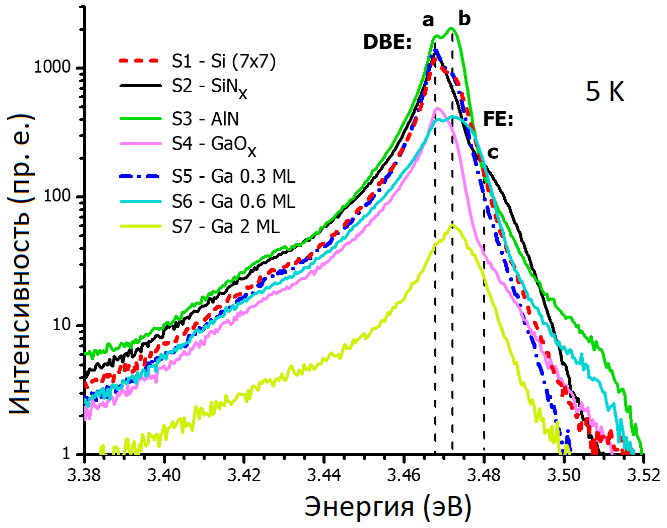
\includegraphics[width=1\linewidth]{Image_30_1}}
	\end{minipage}
	\begin{minipage}[t]{0.47\linewidth}
		\center{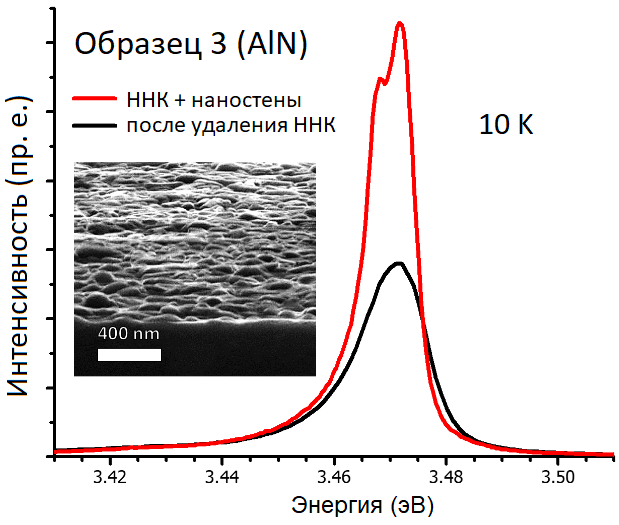
\includegraphics[width=1\linewidth]{Image_30_2}}
	\end{minipage}
\end{frame}

\begin{frame}
	\frametitle{Положение №2}
	\Huge
	Показано, что выбор буферного слоя при МПЭ GaN ННК на Si(111) позволяет
	контролировать морфологию массива. Наиболее однородный по длине и диаметру
	ННК массив с минимальной поверхностной плотностью формируется на затравке
	AlN. Наименее однородный по длине~--- на необработанной подложке c
	реконструкцией Si\((111)7\)\(\times\)\(7\). Массив с наибольшей
	поверхностной плотностью~--- на затравке, полученной в результате нитридации
	реконструкции Si\((111)\sqrt{3}\)\(\times\)\(\sqrt{3} - R30\si{\degree} -
	\text{Ga}\).
\end{frame}

\section{Эпитаксиальные наночастицы GaAs}

\begin{frame}[plain, noframenumbering]
	\begin{center}
		\Huge
		Эпитаксиальные наночастицы GaAs
	\end{center}
\end{frame}

\begin{frame}[c]
	\frametitle{Влияние ростовых параметров на морфологию наночастиц GaAs}
	\centering
	\begin{columns}[onlytextwidth]
		\begin{column}{0.48\textwidth}
			\centering
			\text{Отношение As/Ga}
			\\[10pt]
			\begin{minipage}[t]{0.31\linewidth}
				\center{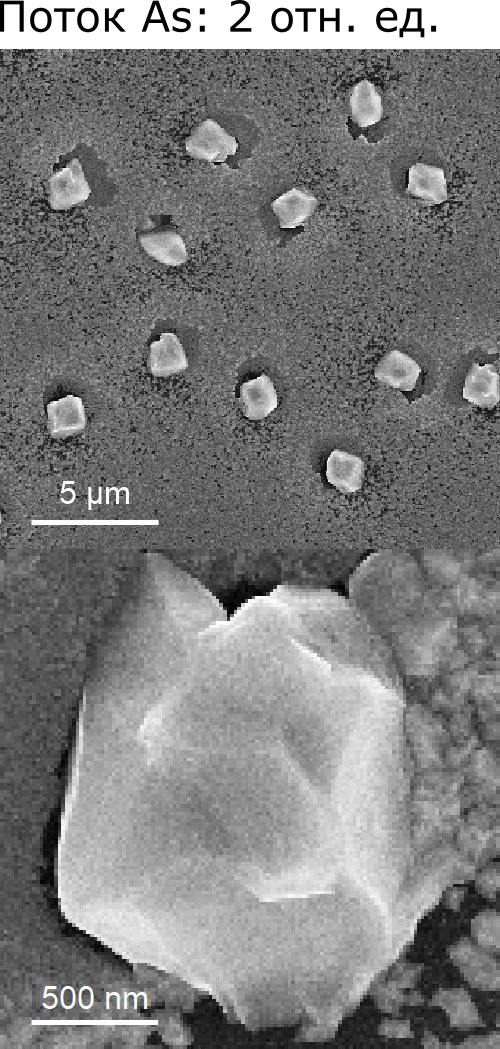
\includegraphics[height=0.38\textheight]{Image_31_1}}
			\end{minipage}
			\begin{minipage}[t]{0.31\linewidth}
				\center{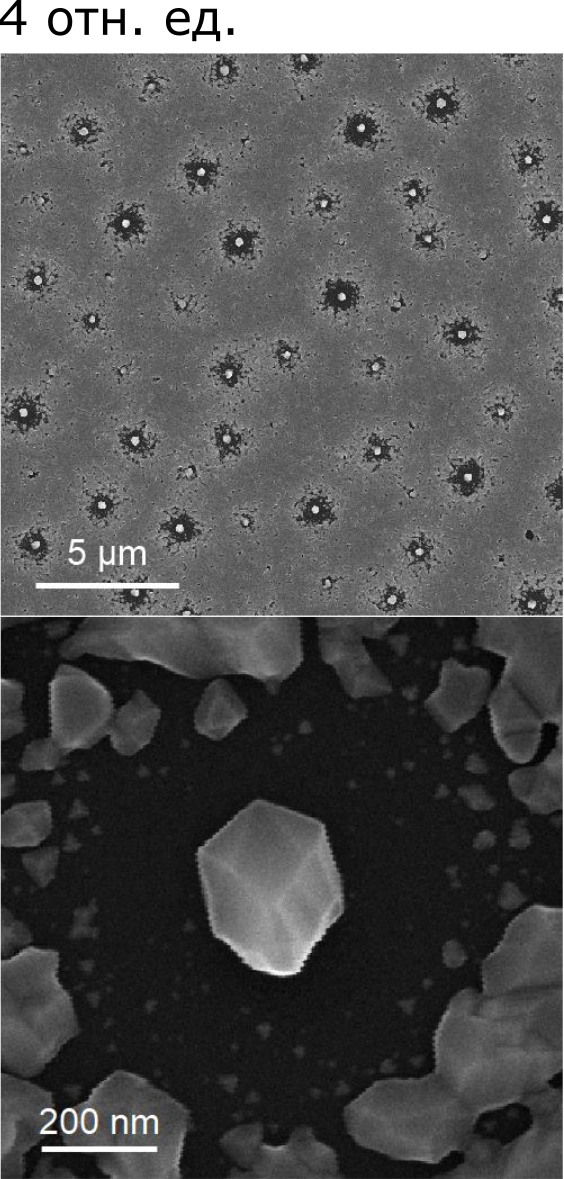
\includegraphics[height=0.38\textheight]{Image_31_2}}
			\end{minipage}
			\begin{minipage}[t]{0.31\linewidth}
				\center{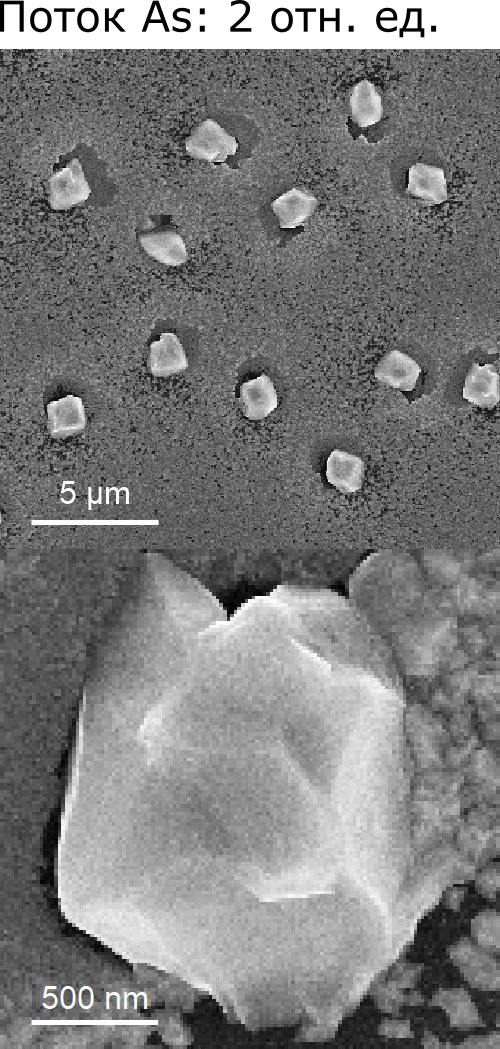
\includegraphics[height=0.38\textheight]{Image_31_1}}
			\end{minipage}
		\end{column}
		\begin{column}{0.48\textwidth}
			\centering
			\text{Температура}
			\\[10pt]
			\begin{minipage}[t]{0.31\linewidth}
				\center{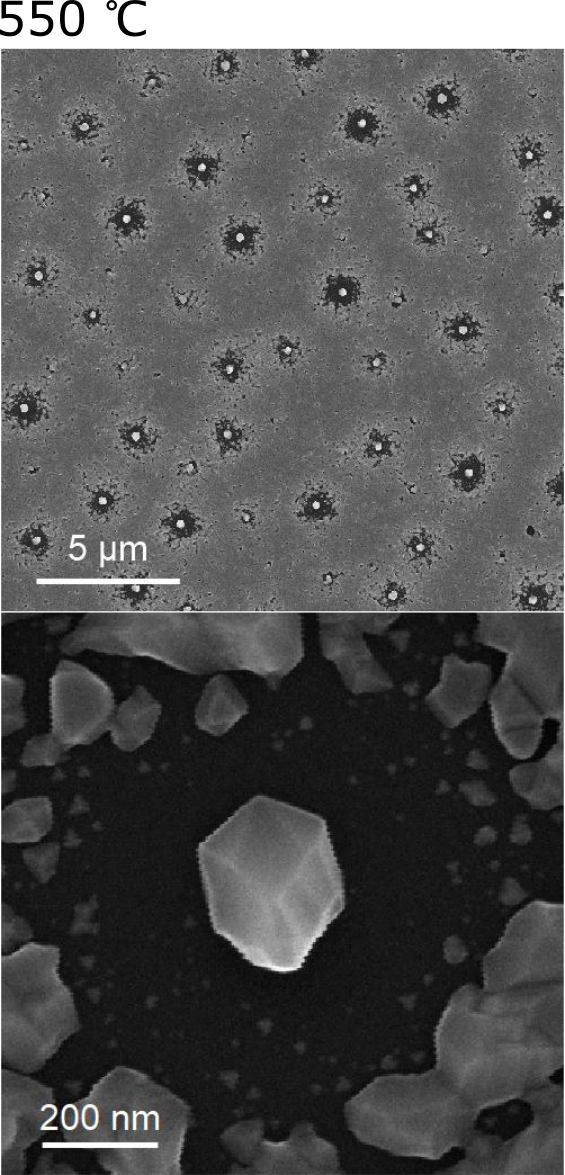
\includegraphics[height=0.38\textheight]{Image_32_1}}
			\end{minipage}
			\begin{minipage}[t]{0.31\linewidth}
				\center{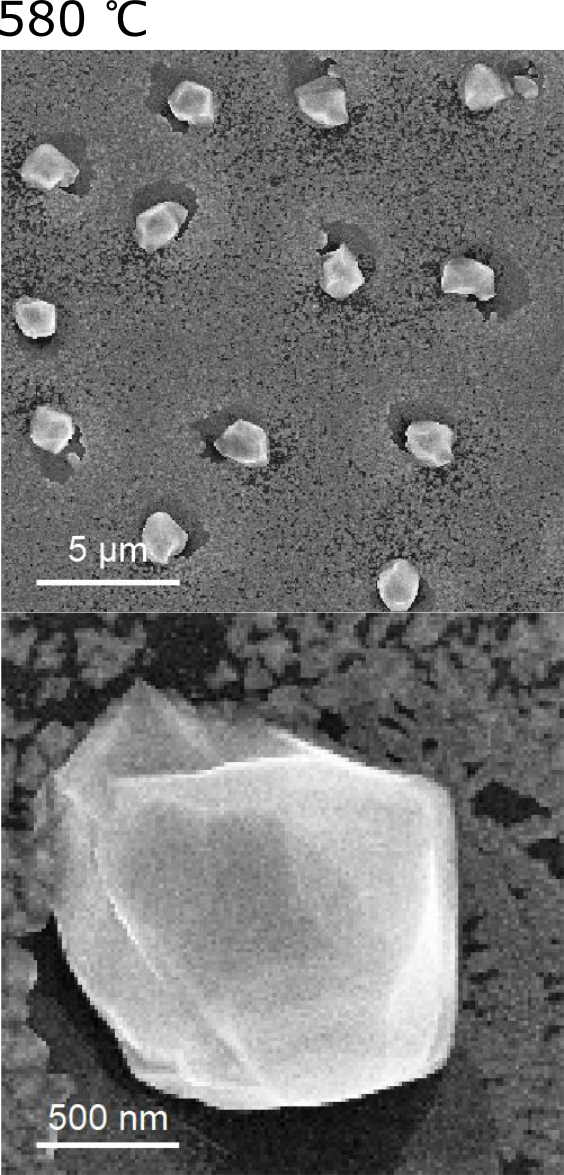
\includegraphics[height=0.38\textheight]{Image_32_2}}
			\end{minipage}
			\begin{minipage}[t]{0.31\linewidth}
				\center{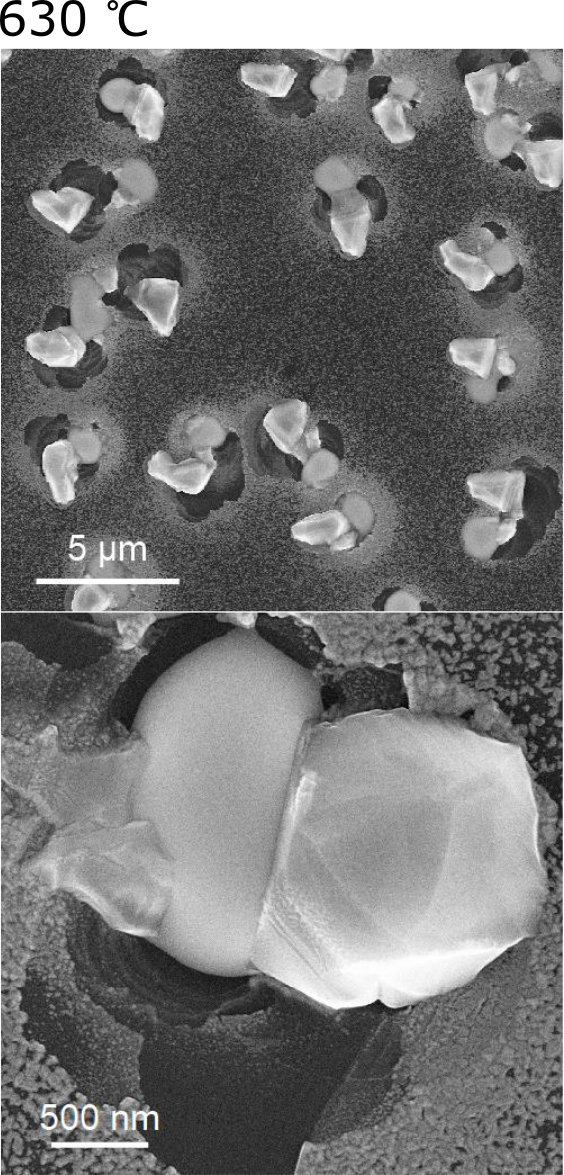
\includegraphics[height=0.38\textheight]{Image_32_3}}
			\end{minipage}
		\end{column}
	\end{columns}
\end{frame}

\begin{frame}
	\frametitle{Изменение морфологии в процессе роста}
	\centering
	\begin{columns}[onlytextwidth]
		\begin{column}{0.48\textwidth}
			\centering
			\text{10 минут роста}
			\\[10pt]
			\begin{minipage}[t]{0.47\linewidth}
				\center{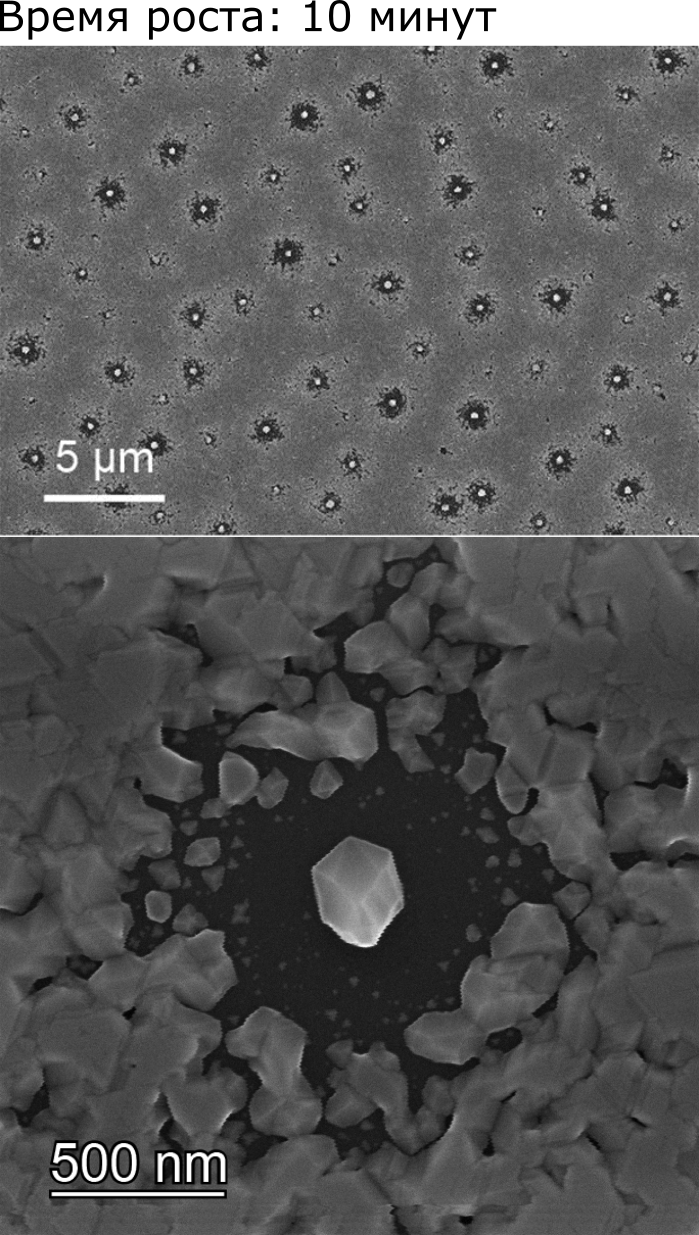
\includegraphics[height=0.49\textheight]{Image_33_1}}
			\end{minipage}
			\begin{minipage}[t]{0.47\linewidth}
				\center{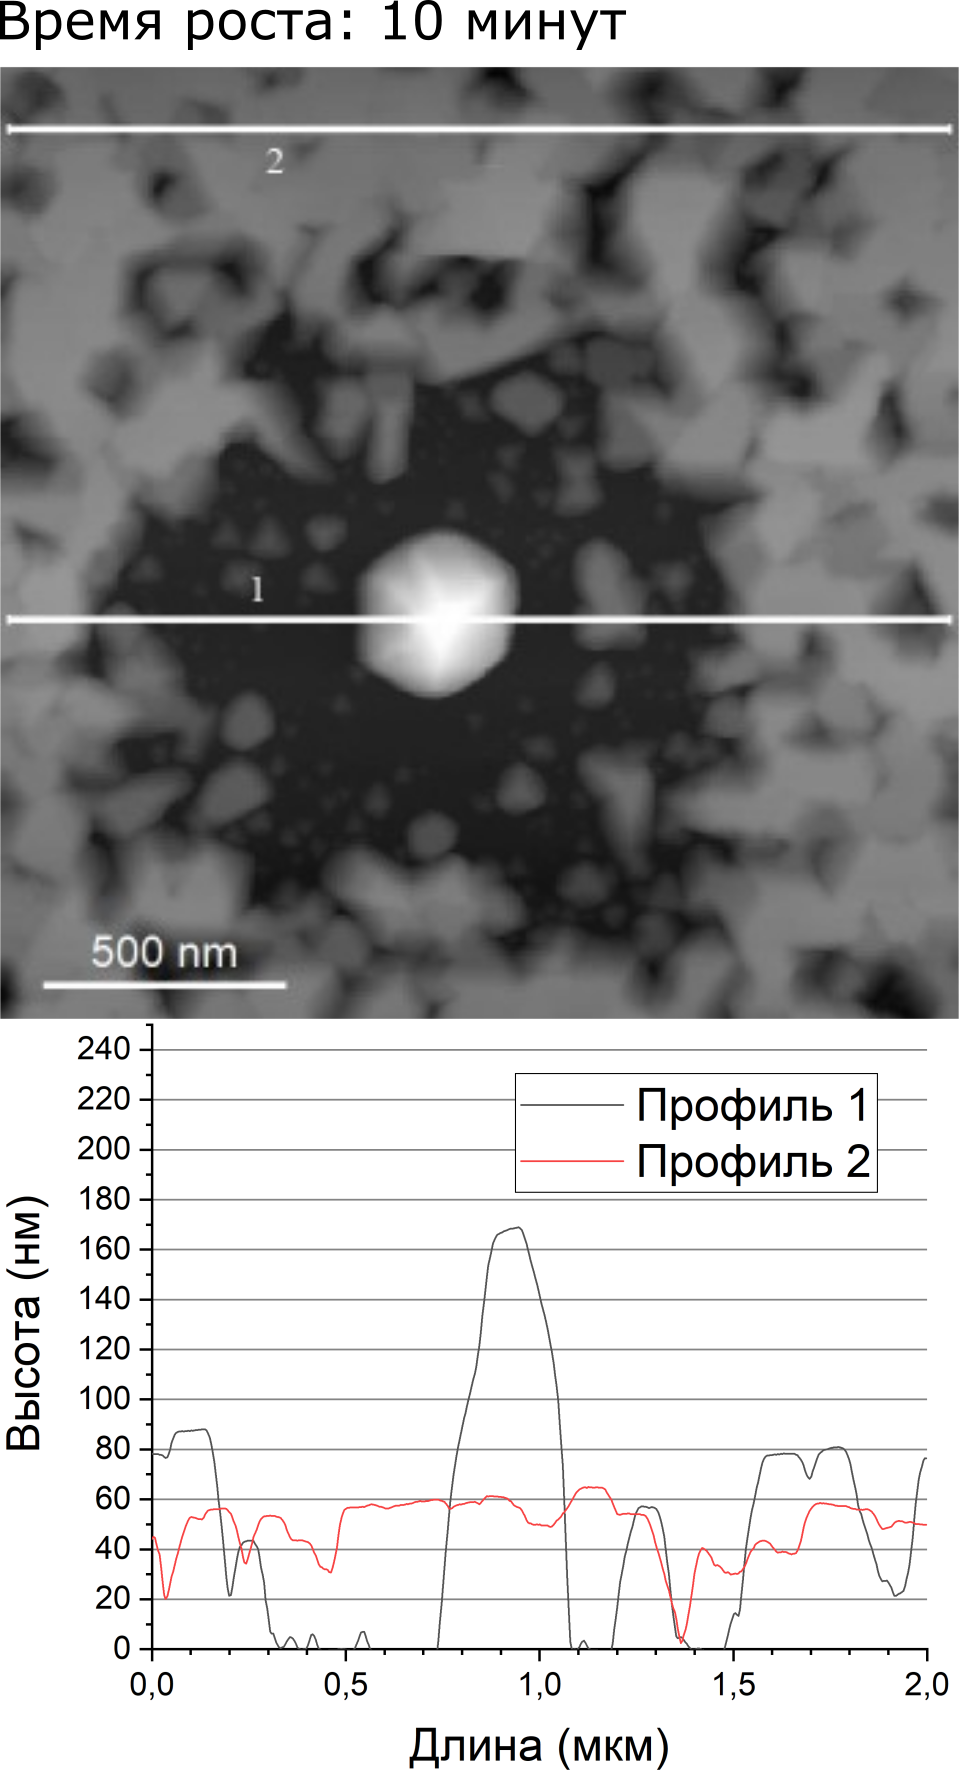
\includegraphics[height=0.49\textheight]{Image_34_1}}
			\end{minipage}
		\end{column}
		\begin{column}{0.47\textwidth}
			\centering
			\text{30 минут роста}
			\\[10pt]
			\begin{minipage}[t]{0.48\linewidth}
				\center{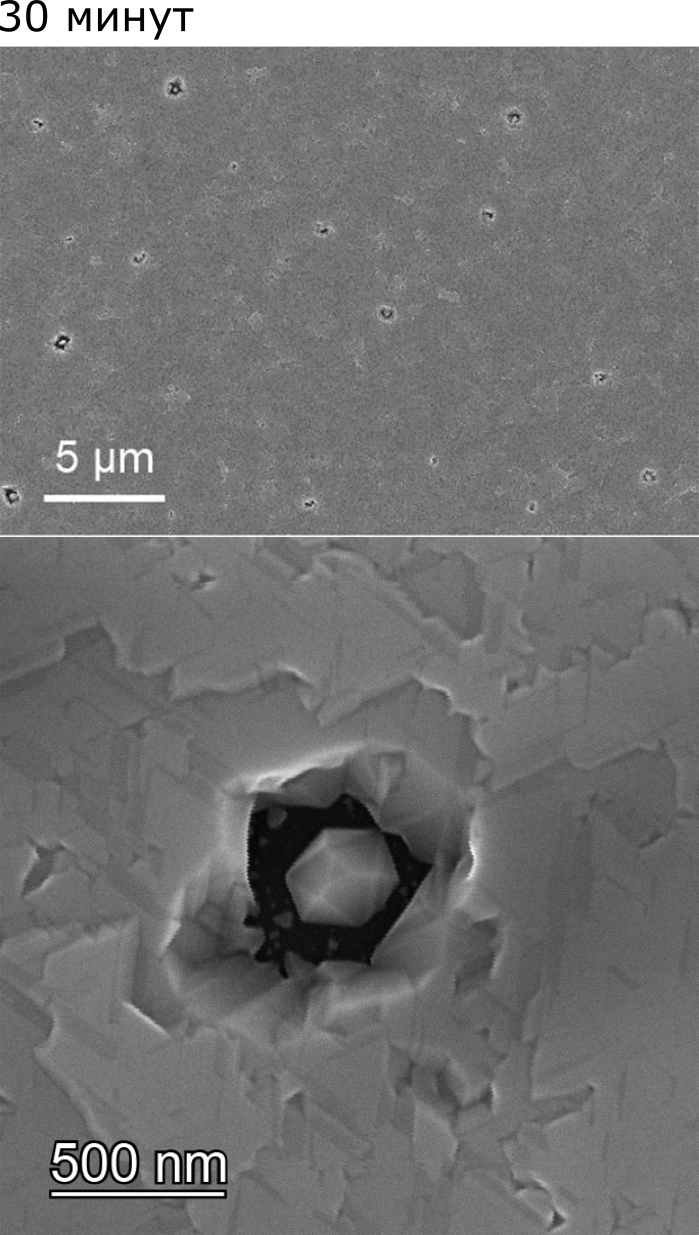
\includegraphics[height=0.49\textheight]{Image_33_2}}
			\end{minipage}
			\begin{minipage}[t]{0.47\linewidth}
				\center{\includegraphics[height=0.49\textheight]{Image_34_2}}
			\end{minipage}
		\end{column}
	\end{columns}
\end{frame}

\begin{frame}
	\frametitle{Огранка GaAs наночастиц}
	\centering
	\includegraphics[height=0.3\textheight]{Image_35_1}
	\includegraphics[height=0.3\textheight]{Image_35_2}
	\\
	\includegraphics[width=0.5\linewidth]{Image_35_3}
\end{frame}

\begin{frame}
	\frametitle{КРС картирование}
	\centering
	\includegraphics[height=0.3\textheight]{Image_36_1}
	\includegraphics[height=0.3\textheight]{Image_36_2}
	\\
	\includegraphics[width=0.5\linewidth]{Image_36_3}
\end{frame}

\begin{frame}
	\frametitle{ФЛ индивидуальных наночастиц GaAs}
	\centering
	\includegraphics[height=0.3\textheight]{Image_36_1}
	\includegraphics[height=0.3\textheight]{Image_36_2}
	\\
	\includegraphics[width=0.5\linewidth]{Image_37}
\end{frame}

\begin{frame}
	\frametitle{Положение №3}
	\large
	Выявлено, что эпитаксиальный синтез GaAs на поверхности Si\((111)\), с
	которой жидкостным методом удалён поверхностный окисел, может приводить к
	формированию наночастиц GaAs по ПЖК механизму. Рост при пониженном отношения
	молекулярных потоков As/Ga или повышенной температуре приводит к увеличению
	диаметра наночастиц в диапазоне от 200~\si{\nano\metre} до
2~\si{\micro\metre}.
\end{frame}

\section{Самокаталитические ННК GaP: кристаллическая структура и влияние условий роста на морфологию массива}

\begin{frame}[plain, noframenumbering]
	\begin{center}
		\Huge
		Самокаталитические ННК GaP: кристаллическая структура и влияние условий роста на морфологию массива
	\end{center}
\end{frame}

\begin{frame}
	\frametitle{Роль подготовки поверхностного оксида}
	\centering
	\hfill
	\includegraphics[width=0.25\linewidth]{Image_38_1}
	\hfill
	\includegraphics[width=0.25\linewidth]{Image_38_2}
	\hfill
	\includegraphics[width=0.25\linewidth]{Image_38_3}
	\hfill
	\bigskip
	\hrule{}
	\bigskip
	\hfill
	\includegraphics[height=0.3\textheight]{Image_39_1}
	\hfill
	\includegraphics[height=0.3\textheight]{Image_39_2}
	\hfill
	\includegraphics[height=0.3\textheight]{Image_39_3}
	\hfill
\end{frame}

\begin{frame}
	\frametitle{Влияние предварительного нанесение Ga}
	\centering
	\includegraphics[width=0.35\linewidth]{Image_40_1}
	\includegraphics[width=0.35\linewidth]{Image_40_2}
\end{frame}


\begin{frame}
	\frametitle{Изменение морфологии массива в процессе роста}
	\centering
	\includegraphics[width=0.35\linewidth]{Image_43_1}
	\includegraphics[width=0.35\linewidth]{Image_43_2}
	\\
	\includegraphics[width=0.35\linewidth]{Image_43_3}
	\includegraphics[width=0.35\linewidth]{Image_43_4}
	\\[5pt]
	\(D_{top}^\ast=\frac{4 \lambda \tan{\varphi}}{\pi f(\vartheta,\varphi)(f_{V/III}-1)}\)
\end{frame}


\begin{frame}
	\frametitle{Влияние отношения ЭДП P/Ga}
	\centering
	\includegraphics[width=0.4\linewidth]{Image_41_1}
	\\
	\includegraphics[width=0.4\linewidth]{Image_41_2}
	\includegraphics[width=0.4\linewidth]{Image_41_3}
\end{frame}


\begin{frame}
	\frametitle{Влияние температуры роста и потока Ga}
	\centering
	\hfill
	\includegraphics[width=0.45\linewidth]{Image_42_1}
	\hfill
	\includegraphics[width=0.45\linewidth]{Image_42_2}
	\hfill
\end{frame}

\begin{frame}
	\frametitle{Влияние изменения условий формирования в процессе роста}
	\centering
	\hfill
	\includegraphics[width=0.45\linewidth]{Image_44_1}
	\hfill
	\includegraphics[width=0.45\linewidth]{Image_44_2}
	\hfill
\end{frame}

\begin{frame}
	\frametitle{РЭМ изображение двухстадийного образца VIII}
	\centering
	\includegraphics[width=0.8\linewidth]{Image_45}
\end{frame}

\begin{frame}
	\frametitle{Кристаллическая структура GaP ННК}
	\centering
	рост 7200~\si{\second} при ЭДП P/Ga 18
	\\
	\includegraphics[width=1\linewidth]{Image_46_1}

	температура роста 640\si{\degreeCelsius};
	\\
	рост 5000~\si{\second} при ЭДП P/Ga 24
	\\
	\includegraphics[width=1\linewidth]{Image_46_2}
	\\
	\includegraphics[width=0.24\linewidth]{Image_46_3}
	\includegraphics[width=0.24\linewidth]{Image_46_4}
	\includegraphics[width=0.24\linewidth]{Image_46_5}
	\includegraphics[width=0.24\linewidth]{Image_46_6}
	\\
	температура роста 640\si{\degreeCelsius};
	\\
	первая стадия: рост 2000~\si{\second} при ЭДП P/Ga 30;
	\\
	вторая стадия: рост 5000~\si{\second} при ЭДП P/Ga 12;
	\\
	\includegraphics[width=1\linewidth]{Image_46_7}
\end{frame}

\begin{frame}
	\frametitle{Положение №4}
	\large
	Установлено, что стабильный диаметр самокаталитических ННК GaP
	определяется отношением молекулярных потоков и температурой. Изменением
	данных параметров в процессе синтеза не нарушает ПЖК механизм роста, что
	дает возможность независимо управлять аспектным отношением и поверхностной
	плотностью ННК GaP.
\end{frame}
